% !TeX program = xelatex
% Overleaf: Menu → Compiler → XeLaTeX  （或使用本目录 latexmkrc）
%
% 换期刊模板时主要改这一段 documentclass / 导言宏包，正文 \cite / \section 可尽量保留。
% Elsevier 例：
%   \documentclass[preprint,12pt]{elsarticle}
% IEEE 例：
%   \documentclass[journal]{IEEEtran}
%
% ctexart 的默认中文字体集 fandol 只支持 XeLaTeX / LuaLaTeX。
% 下面这行让"用错编译器"时直接给出可读的提示，而不是 ctex 的 fontset 报错。
\RequirePackage{iftex}
\RequireXeTeX
\documentclass[UTF8,a4paper,11pt]{ctexart}

\usepackage[margin=2.2cm]{geometry}
\usepackage{amsmath,amssymb,amsfonts,mathtools,bm,amsbsy,amsthm}
\usepackage{graphicx}
\usepackage{pifont}
\usepackage{booktabs,tabularx,array,makecell,multirow}
\usepackage{algorithm}
\usepackage[section]{placeins}
\usepackage{xcolor}
\usepackage{setspace}
\usepackage[backend=biber,style=numeric,sorting=none,maxbibnames=99]{biblatex}
\addbibresource{refs.bib}
\usepackage{hyperref}
\usepackage[nameinlink]{cleveref}

\hypersetup{colorlinks=true,linkcolor=blue,citecolor=blue,urlcolor=blue}
\graphicspath{{figures/}{./}}
\allowdisplaybreaks
\newtheorem{assumption}{假设}
\newtheorem{remark}{注}
\newtheorem{problem}{问题}
\DeclareMathOperator{\diag}{diag}

% MathType AMS-LaTeX 常见残留：多余花括号、array 列格式 *{20}{l}


\title{基于行为克隆增强强化学习的双非合作飞行器三维鲁棒一体化最优规避制导律}
\author{%
梁泰源\textsuperscript{1(\ding{37})},~裴胤\textsuperscript{1},~杨奔\textsuperscript{1}\\[0.6em]
{\normalsize 1.~中国运载火箭技术研究院, 北京 100076, 中国}%
}
\date{}

\begin{document}
\maketitle

\begin{abstract}
传统飞行器规避方法易因过度规避导致终端到达误差过大，而现有考虑目标到达的规避研究多局限于平面单飞行器交会场景。为此，本文建立三维四体相对运动学模型，基于极大值原理推导一体化最优规避与制导律，并通过权重系数协调双非合作飞行器规避、目标到达精度与控制能耗，并利用零控偏差量（zero-effort miss, ZEM）实时估计终端到达性能。针对制导权重的在线优化问题，采用打靶法（shooting method）生成覆盖一定范围初始几何构型的专家轨迹，构建行为克隆增强双延迟深度确定性策略梯度（BC-TD3）框架：先利用专家数据预训练策略网络，再通过强化学习微调，以提高复杂多约束任务下的收敛速度与泛化能力。进一步地，针对角度和角速度测量噪声，设计带稀疏正则化与遗忘因子的递推最小二乘辨识方法，在线估计状态空间模型中的关键非平凡参数，降低噪声对制导指令的影响。300次蒙特卡洛仿真表明，在无噪声条件下，所提BC-TD3方法的双飞行器规避成功率和目标到达成功率分别为94.7\%和94.3\%，优于纯TD3及传统比例导引、程序机动方法；在测量噪声条件下，结合在线辨识后，两项成功率进一步达到96.7\%和96.0\%，与无辨识的纯TD3和程序机动方法成功率进一步拉大，验证了所提方法在三维双非合作飞行器场景中兼顾规避安全性、终端精度与鲁棒性方面的有效性。
\end{abstract}

\noindent\textbf{关键词：} 三维四体运动学；一体化规避与制导；最优控制；深度强化学习；在线参数辨识

\section{引言}
现代空域场景日益呈现多飞行器协同交会特征：两枚或更多非合作飞行器沿刻意错开的交会几何与剩余飞行时间逼近同一指定飞行器\cite{yan2020b,shalumov2019}。对规避方而言，这使规避问题发生了质的变化：增大与其中一枚非合作飞行器终端间隔的机动，可能同时缩小与另一枚的间隔；且每一次机动都会消耗随后用于到达指定目标的控制能力。因此，设计一种在同时面对两枚非合作飞行器时仍保持有效、并兼顾终端精度的规避策略，已成为制导设计的核心问题。

现有规避制导研究大致沿两条主线展开。第一条主线是在改进的制导结构中嵌入规避需求，如面向采用改进比例导引（PN）非合作飞行器的最优规避律\cite{feng2023}、适用于复杂多飞行器场景的有限时间收敛制导律（FTCG）\cite{ding2024}、用于三体交会的协同鲁棒视线（LOS）制导律\cite{luo2023}，以及逃逸距离可控的规避律\cite{yu2023}。第二条主线是将交会过程建模为规避博弈，由博弈最优性条件导出规避方策略\cite{turetsky2003}，并进一步推广到三方高超声速交会\cite{yan2020a}、多方微分对策\cite{liang2022}以及安全关键框架下的协同规避\cite{chen2024}。Shaferman的研究进一步表明，针对采用现代线性制导律的非合作飞行器，可以显式构造近最优规避策略\cite{shaferman2021}，因此可将对方的制导结构视为已知先验信息。然而，上述研究大多以终端间隔为主导目标，甚至将其作为唯一目标，所得制导指令往往使可用法向过载趋于饱和，导致后续的目标到达任务难以完成。

能量感知规避因此受到关注。Li等人针对高超声速变体飞行器提出了节能机动策略\cite{li2024cja}；Zhuang等人将深度强化学习（DRL）应用于六自由度模型，以在姿态稳定性与能耗之间权衡\cite{zhuang2024}；Yao等人则在FTCG律中通过精确时序控制优化能量\cite{yao2024}。Wang等人将终端间隔驱动至给定临界安全值而非最大化，从而限制不必要的控制消耗\cite{wang2024}。规避与继续原任务之间的耦合，已由Qi等人针对受保护目标\cite{qi2017}以及Ren等人通过分层规避—到达策略\cite{ren2025}加以研究。这些工作表明最大规避与终端精度是相互冲突的需求，但其要么只处理单枚非合作飞行器，要么将两个子任务分层解耦，因而两者的交互从未被纳入同一最优性条件。

明确考虑两枚或更多非合作飞行器的研究仍然稀少，并在维数、解的形式或二者上受到限制。Ben-Asher等人在路径角约束下求解了针对两枚非合作飞行器的最优规避，但是平面设定且为开环解\cite{benasher1988}。Shen等人优化了高超声速滑翔飞行器遭遇两枚非合作飞行器时的规避轨迹，同样为离线求解，因而无法响应飞行中的几何扰动\cite{shen2022}。Zhang等人针对多枚轨道非合作飞行器构建了逃逸区，这一几何方法难以适用于剩余飞行时间紧张的大气层末段交会\cite{zhang2023}。Hao等人确实用强化学习研究了双飞行器问题，但其参数化策略建立在二维运动学模型上，无法刻画支配真实三维（3D）交会的面外耦合\cite{hao2025}。目前仍缺乏一种闭环解析制导律，能将规避两枚非合作飞行器、到达目标与控制能耗作为三维空间中的同一耦合优化问题来处理。零控偏差量（zero-effort miss, ZEM）可将线性化交会的终端性能压缩为单一标量\cite{zarchan2019}，并已被证明是反馈制导\cite{guo2013}与逆最优制导\cite{ma2022}的有效综合变量，从而为同时缩减多次交会提供了自然途径。

即便已有解析制导律，其权重系数也无法先验固定：两项规避项、到达项与能量项的相对重要性取决于交会几何，因而权值选取等价于必须沿轨迹求解的非线性优化。深度强化学习适合承担这一任务，已被用于由纯角度测量学习末制导\cite{gaudet2020}、实现无需在线数值优化的计算制导\cite{he2021}，以及处理存在干扰目标时的末制导\cite{deng2023}。确定性策略梯度方法适合此类连续参数调度\cite{lillicrap2016}，而其双延迟变体（TD3）可缓解使朴素形式在多约束下不可靠的价值过估计与策略振荡\cite{fujimoto2018}。然而，从零开始学习样本效率低且易陷入较差局部最优，因此训练中常注入示范数据——通过预填充经验回放缓冲\cite{hester2018,vecerik2017}、将策略更新正则化至示范动作\cite{fujimoto2021}，或对交会数据进行对抗模仿\cite{hu2022,hui2025}。但在现有制导应用中，这类示范多来自启发式规则或其他已学策略，而非底层最优控制问题，其所携带的先验本身并非最优。

另一缺口在于测量的真实性。ZEM动力学的系数是视线角与角速度的函数，若直接由含噪机载传感器输出计算，将产生有偏且相互相关的误差并直接传入制导指令，因此在线估计必不可少\cite{liu2025}。带遗忘因子的递推最小二乘（RLS）是跟踪此类时变系数的标准工具\cite{paleologu2008,bruce2020}，但在某些几何下投影系数激励较弱，无正则化的递推会发生漂移。附加$\ell_1$惩罚可抑制虚假分量并保持递推形式\cite{angelosante2010}，其思路与控制方程的稀疏辨识相一致\cite{brunton2016}。

为弥补上述不足，本文提出了一种面向双非合作飞行器的智能三维规避算法。主要贡献如下。

\begin{enumerate}
\item 建立了三维四体相对运动学模型，将规避与目标到达一体化问题由单非合作飞行器推广到双飞行器，并从原有研究只考虑二维运动学拓展到三维。
\item 设计了同时考虑规避与目标到达的一体化最优制导律，防止过度规避导致目标到达失败。利用极大值原理推出的三维最优制导律充分考虑了规避两非合作飞行器与到达目标等多个任务间存在的耦合，并通过求解$3\times 3$耦合ZEM系统得到闭环解析形式，生成指令无需在线数值优化。
\item 考虑实际应用中存在的测量误差，设计了一种带稀疏正则化与遗忘因子的最小二乘辨识算法，对状态方程矩阵进行结构化辨识，并与制导律闭环，使辨识量替代其解析计算值。
\item 利用打靶法生成考虑各类初始条件的专家轨迹，设计了BC-TD3框架，使用专家轨迹进行预填充后开启强化学习训练，提高多约束复杂任务下的收敛速度与泛化性。在300余次蒙特卡洛仿真中，所提方法在无测量噪声时的双飞行器规避成功率与目标到达成功率分别为94.7\%和94.3\%，结合在线辨识后在有噪声条件下分别达到96.7\%和96.0\%。
\end{enumerate}

本文其余部分安排如下。第2节建立三维四体相对运动学并给出一体化优化问题。第3节给出结构化稀疏遗忘因子递推最小二乘（FF-RLS）辨识方案，第4节推导一体化最优制导律。第5节介绍专家轨迹生成与BC-TD3框架。第6节给出蒙特卡洛仿真结果，第7节总结全文。

\section{问题构建}
\subsection{非线性运动学}
本文针对规避者$A$规避和目标到达场景，考虑在目标T附近部署两个非合作飞行器${D_1}$, ${D_2}$对规避者实施协同逼近。为表述简洁，后文除特殊说明外，统一定义下标$i \in \{ 1,2\} $，其中$i = 1$对应非合作飞行器${D_1}$，$i = 2$对应非合作飞行器${D_2}$。

规避者-目标-非合作飞行器1-非合作飞行器2四体相对运动关系如下图~\ref{fig:fourbody}所示，坐标系OXYZ为以目标T为原点、X轴位于水平面、Y轴竖直向上的地面坐标系。

\begin{figure}[htbp]
\centering
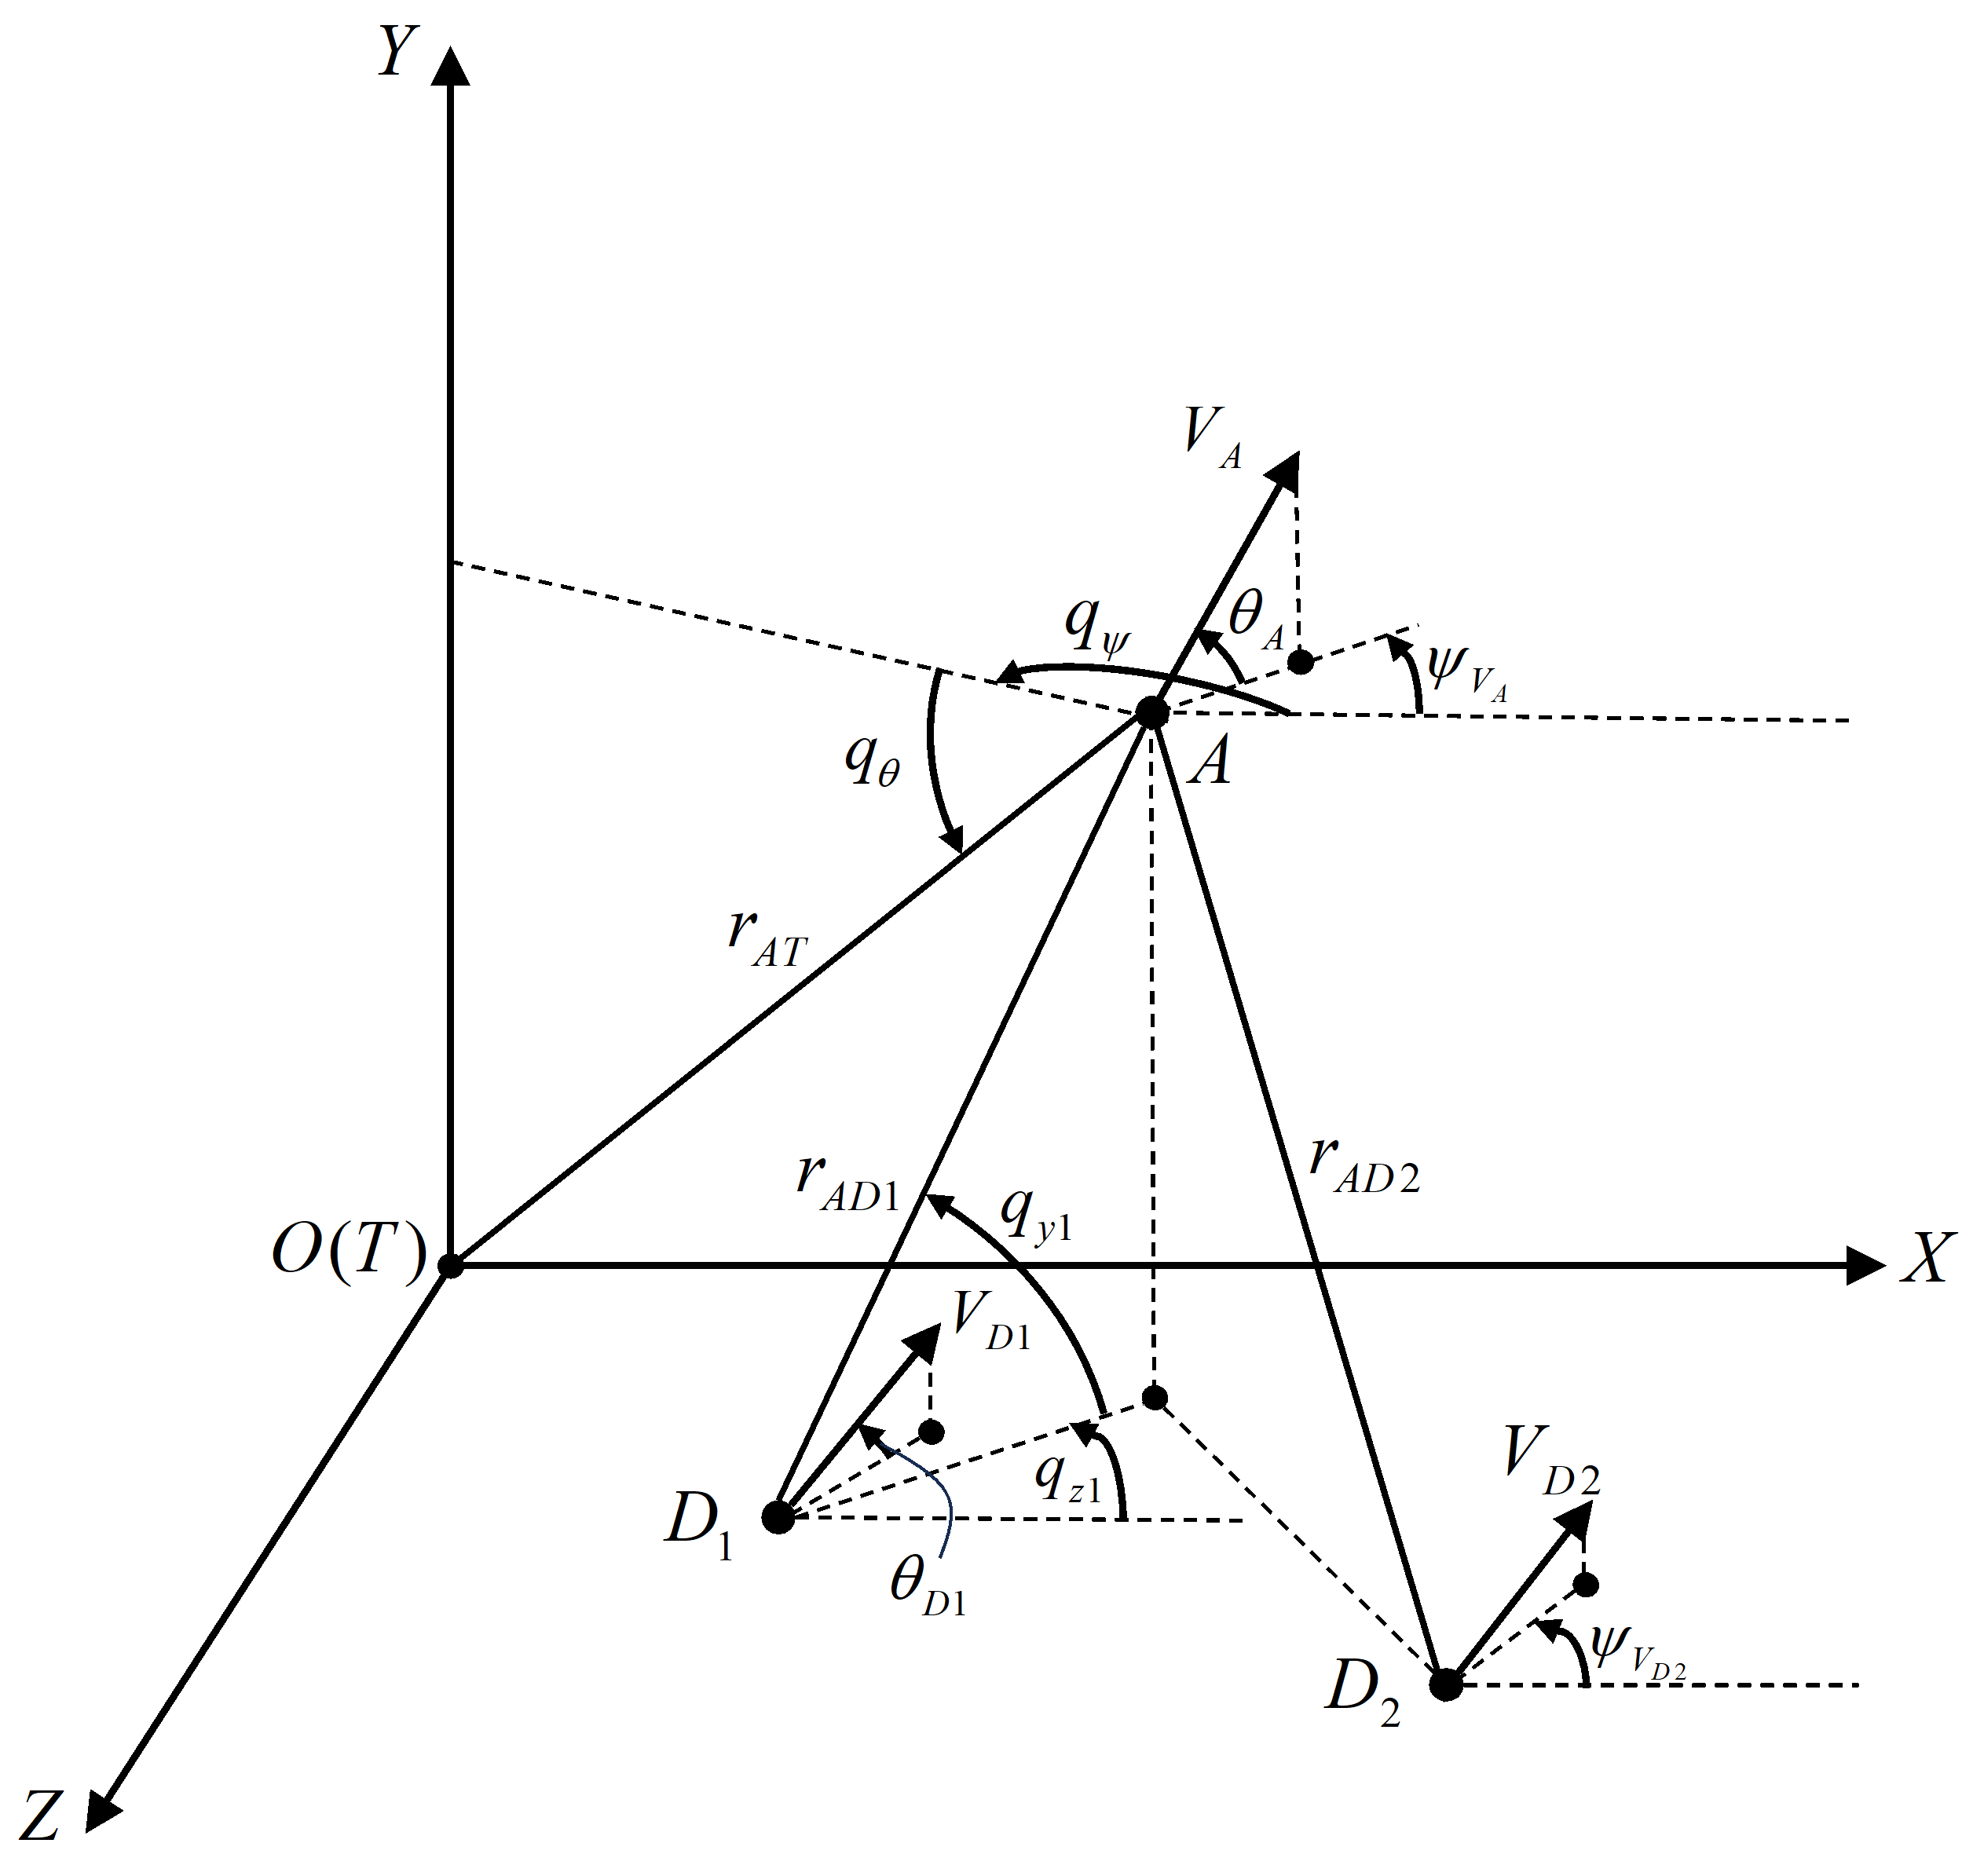
\includegraphics[width=0.92\linewidth]{fig01}
\caption{规避者-目标-非合作飞行器1-非合作飞行器2四体相对运动关系图}
\label{fig:fourbody}
\end{figure}
图~\ref{fig:fourbody}中相对位置和运动关系符号如下表~\ref{tab:symbols}所示。

\begin{table}[htbp]
\centering
\caption{图~\ref{fig:fourbody}相对位置与运动关系符号表}
\label{tab:symbols}
\small
\begin{tabularx}{\linewidth}{lXX}
\toprule
符号 & 含义 & 图~\ref{fig:fourbody}中对应正负 \\
\midrule
${r_{AT}},{r_{ADi}}$ & 规避者与目标、第i个非合作飞行器之间的距离 & 正，正 \\
${q_{yi}},{q_{zi}}$ & 第i个非合作飞行器的俯仰、偏航方向视线角 & 正，正 \\
${q_\theta },{q_\psi }$ & 规避者与目标的俯仰、偏航方向视线角 & 负，正 \\
${V_{Di}},{\theta _{Di}},{\psi _{{V_{Di}}}}$ & 第i个非合作飞行器的速度、航迹倾角和航迹偏角 & 正，正 \\
${V_A},{\theta _A},{\psi _{{V_A}}}$ & 规避者的速度、航迹倾角和航迹偏角 & 正，正 \\
${u_{ri}},{v_{ri}}$ & 规避者加速度、第i枚非合作飞行器加速度在视线坐标系x轴（正方向由第i枚非合作飞行器指向规避者）投影 & 正，正 \\
\bottomrule
\end{tabularx}
\end{table}
非合作飞行器${D_1}$, ${D_2}$与规避者$A$的相对运动方程

\begin{equation}
\label{eq:1}
\left\{ {\begin{array}{*{20}{l}}
  \begin{aligned}
& {{\dot r}_{ADi}} =  - {V_{Di}}\left[ {\cos {\theta _{Di}}\cos {q_{yi}}\cos \left( {{q_{zi}} - {\psi _{{V_{Di}}}}} \right) + \sin {\theta _{Di}}\sin {q_{yi}}} \right] +  \\
& {\text{   }}{V_A}\left[ {\cos {\theta _A}\cos {q_{yi}}\cos \left( {{q_{zi}} - {\psi _{{V_A}}}} \right) + \sin {\theta _A}\sin {q_{yi}}} \right]
\end{aligned} \\
  \begin{aligned}
& {{\dot q}_{yi}}{r_{ADi}} = {V_{Di}}\left[ {\cos {\theta _{Di}}\sin {q_{yi}}\cos \left( {{q_{zi}} - {\psi _{{V_{Di}}}}} \right) - \sin {\theta _{Di}}\cos {q_{yi}}} \right] -  \\
& {V_A}\left[ {\cos {\theta _A}\sin {q_{yi}}\cos \left( {{q_{zi}} - {\psi _{{V_A}}}} \right) - \sin {\theta _A}\cos {q_{zi}}} \right]
\end{aligned} \\
  \begin{aligned}
& {{\dot q}_{zi}}{r_{ADi}}\cos {q_{yi}} = {V_{Di}}\cos {\theta _{Di}}\sin \left( {{q_{yi}} - {\psi _{{V_{Di}}}}} \right) -  \\
& {\text{           }}{V_A}\cos {\theta _A}\sin \left( {{q_{zi}} - {\psi _{{V_A}}}} \right)
\end{aligned}
\end{array}} \right.
\end{equation}
规避者和目标相对运动方程

\begin{equation}
\label{eq:2}
\left\{ {\begin{array}{*{20}{l}}
  {{{\dot r}_{AT}} = {V_A}\left[ {\sin {q_\theta }\sin {\theta _A} - \cos \left( {{q_\psi } - {\psi _{{V_A}}}} \right)\cos {q_\theta }\cos {\theta _A}} \right]} \\ 
  {{{\dot q}_\theta } = \frac{{{V_A}\left[ {\cos {\theta _A}\sin {q_\theta }\cos \left( {{q_\psi } - {\psi _{{V_A}}}} \right) - \sin {\theta _A}\cos {q_\theta }} \right]}}{{{r_{AT}}}}} \\ 
  {{{\dot q}_\psi } = \frac{{{V_A}\cos {\theta _A}\cos \left( {{q_\psi } - {\psi _{{V_A}}}} \right)}}{{{r_{AT}}\cos {q_\theta }}}} 
\end{array}} \right.
\end{equation}
由运动学关系可得非合作飞行器与规避者视线方向相对加速度

\begin{equation}
\label{eq:3}
{\ddot r_{ADi}} = {r_{ADi}}\dot q_{yi}^2 + {r_{ADi}}\dot q_{zi}^2{\cos ^2}{q_{yi}} + {u_{ri}} - {v_{ri}}
\end{equation}
式中，${u_{ri}},{v_{ri}}$分别为规避者和第i个非合作飞行器的加速度在非合作飞行器与规避者视线坐标系（设为视线坐标系${S_i}$）x轴投影，坐标系x轴正向定义为非合作飞行器指向规避者。

目标与规避者视线方向相对加速度

\begin{equation}
\label{eq:4}
{\ddot r_{AT}} = {r_{AT}}\dot q_\theta ^2 + {r_{AT}}\dot q_\psi ^2{\cos ^2}{q_\theta } + {u_{rT}}
\end{equation}
式中，${u_{rT}}$为规避者加速度在目标与规避者视线坐标系（设为视线坐标系${S_T}$）x轴投影，坐标系x轴正向定义为目标指向规避者。

对每个飞行器，三维运动学方程为:

\begin{equation}
\label{eq:5}
\left\{ {\begin{array}{*{20}{l}}
  {{{\dot x}_j} = {V_j}\cos {\theta _j}\cos {\psi _{{V_j}}}} \\ 
  {{{\dot y}_j} = {V_j}\sin {\theta _j}} \\ 
  {{{\dot z}_j} =  - {V_j}\cos {\theta _j}\sin {\psi _{{V_j}}}} \\ 
  {{{\dot \theta }_j} = \frac{{{a_{yj}}}}{{{V_j}}}} \\ 
  {{{\dot \psi }_j} =  - \frac{{{a_{zj}}}}{{{V_j}\cos {\theta _j}}}} 
\end{array},j = A,{D_1}.{D_2}} \right.
\end{equation}
式中，$({x_i},{y_i},{z_i})$为飞行器在地面坐标系位置坐标；${a_{yj}}$, ${a_{zj}}$分别表示垂直于飞行器速度矢量的铅垂方向和水平方向的法向加速度。

由视线方向相对加速度关系式可知，规避者与第i枚非合作飞行器的加速度在视线坐标系${S_i}$的x轴投影${u_{ri}}$和${v_{ri}}$，与各自法向加速度${a_{yA}}$,${a_{zA}}$和${a_{yDi}}$,${a_{zDi}}$存在坐标转换关系。设地面坐标系到视线坐标系${S_i}$的转换矩阵为${\mathbf{L}}({q_{yi}},{q_{zi}})$，地面坐标系到航迹坐标系的转换矩阵为${\mathbf{L}}(\theta ,{\psi _V})$，则两者的投影关系可表示为

\begin{equation}
\label{eq:6}
{u_{ri}} = \left[ {\begin{array}{*{20}{c}}
  1&0&0 
\end{array}} \right]{\mathbf{L}}({q_{yi}},{q_{zi}}){{\mathbf{L}}^{ - 1}}({\theta _A},{\psi _{{V_A}}})\left[ {\begin{array}{*{20}{c}}
  0 \\ 
  {{a_{yA}}} \\ 
  {{a_{zA}}} 
\end{array}} \right]
\end{equation}
\begin{equation}
\label{eq:7}
{v_{ri}} = \left[ {\begin{array}{*{20}{c}}
  1&0&0 
\end{array}} \right]{\mathbf{L}}({q_{yi}},{q_{zi}}){{\mathbf{L}}^{ - 1}}({\theta _{Di}},{\psi _{{V_{Di}}}})\left[ {\begin{array}{*{20}{c}}
  0 \\ 
  {{a_{yDi}}} \\ 
  {{a_{zDi}}} 
\end{array}} \right]
\end{equation}
其中转换矩阵的具体形式与三维空间坐标系转换的通用定义一致，此处不再赘述。同理，设地面坐标系到视线坐标系${S_T}$的转换矩阵为${\mathbf{L}}({q_\theta },{q_\psi })$，则规避者与目标的加速度在坐标系${S_T}$的x轴投影

\begin{equation}
\label{eq:8}
{u_{rT}} = \left[ {\begin{array}{*{20}{c}}
  1&0&0 
\end{array}} \right]{\mathbf{L}}({q_\theta },{q_\psi }){{\mathbf{L}}^{ - 1}}({\theta _A},{\psi _{{V_A}}})\left[ {\begin{array}{*{20}{c}}
  0 \\ 
  {{a_{yA}}} \\ 
  {{a_{zA}}} 
\end{array}} \right]
\end{equation}
\begin{assumption}
非合作飞行器均采用经典比例导引（PN）制导律，其加速度指令为：
\end{assumption}
\begin{equation}
\label{eq:9}
\left[ {\begin{array}{*{20}{c}}
  {{a_{yDi}}} \\ 
  {{a_{zDi}}} 
\end{array}} \right] = \left[ {\begin{array}{*{20}{c}}
  {{K_{Di}}{V_{Di}}{{\dot q}_{yi}}} \\ 
  { - {K_{Di}}{V_{Di}}{{\dot q}_{zi}}\cos {\theta _{Di}}} 
\end{array}} \right]
\end{equation}
式中，${K_{Di}}$为第i枚非合作飞行器比例导引系数。

\begin{assumption}
两个非合作飞行器性能指标相同，即${K_{{D_1}}} = {K_{{D_2}}} = {K_D}$, ${V_{{D_1}}} = {V_{{D_2}}} = {V_D}$，以及期望规避距离满足$d_1^* = d_2^* = {d^*}$.
\end{assumption}
\subsection{线性化状态空间模型}
将式\eqref{eq:6}、\eqref{eq:7}及其中的转换矩阵代入式\eqref{eq:3}得

\begin{equation}
\label{eq:10}
\begin{gathered}
  {{\ddot r}_{ADi}} = {r_{ADi}}\left( {\dot q_{yi}^2 + \dot q_{zi}^2{{\cos }^2}{q_{yi}}} \right) - \cos {q_{yi}}\sin \left( {{q_{zi}} - {\psi _{{V_A}}}} \right){a_{zA}} +  \\ 
  {a_{yA}}\left[ { - \cos {q_{yi}}\sin {\theta _A}\cos \left( {{q_{zi}} - {\psi _{{V_A}}}} \right) + \sin {q_{yi}}\cos {\theta _A}} \right] -  \\ 
  {a_{yDi}}\left[ { - \cos {q_{yi}}\sin {\theta _{Di}}\cos \left( {{q_{zi}} - {\psi _{{V_{Di}}}}} \right) + \sin {q_{yi}}\cos {\theta _{Di}}} \right] +  \\ 
  \cos {q_{yi}}\sin \left( {{q_{zi}} - {\psi _{{V_{Di}}}}} \right){a_{zDi}} \\ 
\end{gathered}
\end{equation}
同理，将式\eqref{eq:8}及其中的转换矩阵代入式\eqref{eq:4}得

\begin{equation}
\label{eq:11}
\begin{gathered}
  {{\ddot r}_{AT}} = {r_{AT}}\left( {\dot q_\theta ^2 + \dot q_\psi ^2{{\cos }^2}{q_\theta }} \right) + (\cos {q_\theta }\cos {q_\psi }\sin {\theta _A} + \sin {q_\theta }\cos {\theta _A}){a_{yA}} +  \\ 
  {a_{zA}}(\sin {\theta _A}\sin {\psi _{{V_A}}}\sin {q_\theta } - \cos {\theta _A}\sin {\psi _{{V_A}}}\cos {q_\theta }\cos {q_\psi } - \cos {\psi _{{V_A}}}\cos {q_\theta }\sin {q_\psi }) \\ 
\end{gathered}
\end{equation}
定义状态变量${x_i} = {\left[ {\begin{array}{*{20}{c}}
  {{r_{ADi}}}&{{{\dot r}_{ADi}}} 
\end{array}} \right]^T}$，控制变量\[{u_A} = {\left[ {\begin{array}{*{20}{c}}
  {{a_{yA}}}&{{a_{zA}}} 
\end{array}} \right]^T}\]，则可得规避者与第i个非合作飞行器交互的状态空间方程

\begin{equation}
\label{eq:12}
\mathop {{x_i}}\limits^. (t) = {{\mathbf{A}}_i}{x_i}(t) + {{\mathbf{B}}_i}{u_A}(t) + {{\mathbf{C}}_i} + {v_i}
\end{equation}
式中，\[{{\mathbf{A}}_i} = \left[ {\begin{array}{*{20}{c}}
  0&1 \\ 
  {\dot q_{yi}^2 + \dot q_{zi}^2{{\cos }^2}{q_{yi}}}&0 
\end{array}} \right]\],${{\mathbf{B}}_i} = \left[ {\begin{array}{*{20}{c}}
  0&0 \\ 
  {{B_{1i}}}&{{B_{2i}}} 
\end{array}} \right]$,${{\mathbf{C}}_i} = \left[ {\begin{array}{*{20}{c}}
  0 \\ 
  {{C_{1i}}} 
\end{array}} \right]$，其中

\begin{equation}
\label{eq:13}
\left\{ {\begin{array}{*{20}{l}}
  {{B_{1i}} = \sin {q_{yi}}\cos {\theta _A} - \cos {q_{yi}}\sin {\theta _A}\cos \left( {{q_{zi}} - {\psi _{{V_A}}}} \right)} \\ 
  {{B_{2i}} = \cos {q_{yi}}\sin \left( {{q_{zi}} - {\psi _{{V_A}}}} \right)} \\ 
  {{C_{1i}} = \cos {q_{yi}}\sin \left( {{q_{zi}} - {\psi _{{V_{Di}}}}} \right){a_{zDi}} + [\cos {q_{yi}}\sin {\theta _{Di}}\cos \left( {{q_{zi}} - {\psi _{{V_{Di}}}}} \right) - \sin {q_{yi}}\cos {\theta _{Di}}]{a_{yDi}}} 
\end{array}} \right.
\end{equation}
定义状态变量${x_{AT}} = {\left[ {\begin{array}{*{20}{c}}
  {{r_{AT}}}&{{{\dot r}_{AT}}} 
\end{array}} \right]^T}$，则可得规避者与目标的相对状态空间方程

\begin{equation}
\label{eq:14}
{\dot x_{AT}}(t) = {{\mathbf{A}}_T}{x_{AT}}(t) + {{\mathbf{B}}_T}{u_A}(t)
\end{equation}
式中，\[{{\mathbf{A}}_T} = \left[ {\begin{array}{*{20}{c}}
  0&1 \\ 
  {\dot q_\theta ^2 + \dot q_\psi ^2{{\cos }^2}{q_\theta }}&0 
\end{array}} \right]\],${{\mathbf{B}}_T} = \left[ {\begin{array}{*{20}{c}}
  0&0 \\ 
  {{B_{1T}}}&{{B_{2T}}} 
\end{array}} \right]$，其中

\begin{equation}
\label{eq:15}
\left\{
\begin{aligned}
& {B_{1T}} = \cos {q_\theta }\cos {q_\psi }\sin {\theta _A} + \sin {q_\theta }\cos {\theta _A} \\
& {B_{2T}} = \sin {\theta _A}\sin {\psi _{{V_A}}}\sin {q_\theta } - \cos {\theta _A}\sin {\psi _{{V_A}}}\cos {q_\theta }\cos {q_\psi } - \cos {\psi _{{V_A}}}\cos {q_\theta }\sin {q_\psi }
\end{aligned}
\right.
\end{equation}
\begin{remark}
系统\eqref{eq:12}-\eqref{eq:15}是线性时变的(LTV)，但在每个离散制导周期内，矩阵${{\mathbf{A}}_i}$, ${{\mathbf{B}}_i}$, ${{\mathbf{C}}_i}$, ${{\mathbf{A}}_T}$, ${{\mathbf{B}}_T}$可近似视为时不变。该拟冻结系数假设在工程实践中已得到广泛验证，并为第3节的在线参数辨识提供了数学基础。
\end{remark}
辨识目标汇总. 待辨识的非平凡元素如表~\ref{tab:nontrivial}所示：

\begin{table}[htbp]
\centering
\caption{待辨识非平凡元素}
\label{tab:nontrivial}
\small
\begin{tabularx}{\linewidth}{lXXX}
\toprule
方程 & 矩阵 & 元素 & 物理含义 \\
\midrule
式\eqref{eq:12} & ${{\mathbf{A}}_i}$ & $A_{21}^{(i)} = \dot q_{yi}^2 + \dot q_{zi}^2{\cos ^2}{q_{yi}}$ & 视线角速率耦合 \\
式\eqref{eq:12} & ${B_i}$ & ${B_{1i}},{B_{2i}}$ & 规避者加速度投影系数（非合作飞行器方向） \\
式\eqref{eq:12} & ${C_i}$ & ${C_i}$ & 非合作飞行器机动加速度偏置 \\
式\eqref{eq:15} & ${{\mathbf{A}}_T}$ & $A_{21}^{(T)} = \dot q_\theta ^2 + \dot q_\psi ^2{\cos ^2}{q_\theta }$ & 目标-规避者视线角速率耦合 \\
式\eqref{eq:15} & ${B_T}$ & ${B_{1T}},{B_{2T}}$ & 规避者加速度投影系数（目标方向） \\
\bottomrule
\end{tabularx}
\end{table}
\begin{remark}
a（测量噪声）. 在实际应用中，式\eqref{eq:13}和\eqref{eq:15}中的矩阵元素由机载传感器/IMU测量得到，而非由无噪声理想运动学计算。测量得到的视线角、视线角速率与飞行器航迹倾角/航向角均叠加零均值高斯白噪声：
\end{remark}
\begin{equation}
\label{eq:16}
\begin{gathered}
  {{\tilde q}_\alpha } = {q_\alpha } + {\nu _{q,\alpha }},\quad {\nu _{q,\alpha }}\sim \mathcal{N}(0,\sigma _q^2), \hfill \\
  {{\tilde \dot q}_\alpha } = {{\dot q}_\alpha } + {\nu _{\dot q,\alpha }},\quad {\nu _{\dot q,\alpha }}\sim \mathcal{N}(0,\sigma _{\dot q}^2), \hfill \\
  {{\tilde \theta }_j} = {\theta _j} + {\nu _{\theta ,j}},\quad {\nu _{\theta ,j}}\sim \mathcal{N}(0,\sigma _\theta ^2), \hfill \\
  {{\tilde \psi }_{{V_j}}} = {\psi _{{V_j}}} + {\nu _{\psi ,j}},\quad {\nu _{\psi ,j}}\sim \mathcal{N}(0,\sigma _\psi ^2), \hfill \\ 
\end{gathered}
\end{equation}
式中，$\alpha  \in \left\{ {{y_i},{z_i},\theta ,\psi } \right\}$分别对应与NCV（非合作飞行器）视线和与目标视线各通道，$j \in \left\{ {A,{D_1},{D_2}} \right\}$. 该传感器噪声模型即为第3节在线参数辨识框架的出发点，该框架从相对距离动力学中恢复矩阵元素，而不依赖对噪声敏感的解析式\eqref{eq:13}/\eqref{eq:15}。

\subsection{最优问题建立}
为降低系统阶次并简化求解，引入ZEM $z(t)$。定义规避者与第i个非合作飞行器的ZEM

\begin{equation}
\label{eq:17}
{z_i}(t) = \left[ {\begin{array}{*{20}{c}}
  1&0 
\end{array}} \right]\Omega \left( {{t_{fi}},t} \right){x_i}(t)
\end{equation}
式中，状态转移矩阵

\begin{equation}
\label{eq:18}
\Omega \left( {{t_{fi}},t} \right) = {e^{{A_i}\left( {{t_{fi}} - t} \right)}} = \left[ {\begin{array}{*{20}{c}}
  {\cosh ({{\dot Q}_i}{t_{{\text{go,i}}}})}&{\frac{{\sinh ({{\dot Q}_i}{t_{{\text{go,i}}}})}}{{{{\dot Q}_i}}}} \\ 
  {{{\dot Q}_i}\sinh ({{\dot Q}_i}{t_{{\text{go,i}}}})}&{\cosh ({{\dot Q}_i}{t_{{\text{go,i}}}})} 
\end{array}} \right]
\end{equation}
其中，${\dot Q_i} = \sqrt {\dot q_{yi}^2 + \dot q_{zi}^2{{\cos }^2}{q_{yi}}} $为视线角速度合成量，${t_{go,i}} = {t_{fi}} - t$为剩余飞行时间。利用状态转移矩阵性质$\dot \Omega \left( {{t_{fi}},t} \right) =  - \Omega \left( {{t_{fi}},t} \right){A_i}$，对式\eqref{eq:17}求导整理可得

\begin{equation}
\label{eq:19}
{\dot z_i}(t) = {\varphi _i}(t)b_i^T{u_A}(t) - {\varphi _i}(t){v_{ri}}
\end{equation}
式中，

\begin{equation}
\label{eq:20}
\left\{
\begin{aligned}
& {\varphi _i}(t) = \frac{{{e^{{{\dot Q}_i}{t_{go,i}}}} - {e^{ - {{\dot Q}_i}{t_{go,i}}}}}}{{2{{\dot Q}_i}}} \\
& {b_i} = {\left[ {\begin{array}{*{20}{c}}
  {{B_{1i}}}&{{B_{2i}}}
\end{array}} \right]^T}
\end{aligned}
\right.
\end{equation}
同理可得规避者与目标的ZEM导数

\begin{equation}
\label{eq:21}
{\dot z_T}(t) = {\varphi _T}(t)b_t^T{u_A}(t)
\end{equation}
式中，

\begin{equation}
\label{eq:22}
\left\{
\begin{aligned}
& {\varphi _T}(t) = \frac{{{e^{{{\dot Q}_T}{t_{go,T}}}} - {e^{ - {{\dot Q}_T}{t_{go,T}}}}}}{{2{{\dot Q}_T}}} \\
& {b_t} = {\left[ {\begin{array}{*{20}{c}}
  {{B_{1T}}}&{{B_{2T}}}
\end{array}} \right]^T}
\end{aligned}
\right.
\end{equation}
其中，${\dot Q_T} = \sqrt {\dot q_\theta ^2 + \dot q_\psi ^2{{\cos }^2}{q_\theta }} $,${t_{go,T}} = {t_{fT}} - t$.

本文智能规避算法的核心目标是在保证成功规避两枚非合作飞行器的同时，最小化机动能量消耗，并避免过度机动影响后续目标到达。为此，构建如下二次型性能指标函数

\begin{equation}
\label{eq:23}
\mathop {\min }\limits_{{u_A}} J = \sum\nolimits_{i = 1}^2 {\frac{{{w_i}}}{2}{{\left[ {z\left( {{t_{fi}}} \right) - d_i^*} \right]}^2}}  + \frac{{{w_E}}}{2}\int_{{t_0}}^{{t_f}} {u_A^T{u_A}d\tau {\text{ + }}\frac{{{w_T}}}{2}z_T^2\left( {{t_{fT}}} \right)}
\end{equation}
式中，${w_i} > 0$为规避ZEM权重，${w_E} > 0$为控制能量权重，${w_T} > 0$为目标到达ZEM权重，$d_i^*$为规避者与第i个非合作飞行器的期望规避距离，通常设定为略大于非合作飞行器作用半径。${t_f} = \max ({t_{f1}},{t_{f2}})$为全局规避终止时刻。为体现对两枚非合作飞行器的均衡规避需求，设${w_1} + {w_2} = w$（$w$为一正常数），且${w_1}$, ${w_2}$满足

\begin{equation}
\label{eq:24}
\left\{
\begin{aligned}
& {w_1} = w \cdot \frac{1}{{1 + {e^{ - \gamma }}}} \\
& {w_2} = w - {w_1} = w \cdot \frac{{{e^{ - \gamma }}}}{{1 + {e^{ - \gamma }}}}
\end{aligned}
\right.
\end{equation}
\begin{problem}[一体化最优规避与制导]
给定状态空间方程\eqref{eq:12}与\eqref{eq:14}，在运动学\eqref{eq:1}–\eqref{eq:5}约束下，求使性能指标\eqref{eq:23}最小的最优控制$u_A^*(t)$。
\end{problem}

\section{在线参数辨识}
\subsection{参数辨识问题构建}
根据状态空间方程\eqref{eq:12}和\eqref{eq:14}，每个方程的第二行包含非平凡元素。对于规避者-非合作飞行器对，从方程\eqref{eq:10}中提取二阶动力学：

\begin{equation}
\label{eq:25}
{\ddot r_{ADi}}(t) = \underbrace {(\dot q_{yi}^2 + \dot q_{zi}^2{{\cos }^2}{q_{yi}})}_{A_{21}^{(i)}} \cdot {r_{A{D_i}}}(t) + {B_{1i}} \cdot {a_{yA}}(t) + {B_{2i}} \cdot {a_{zA}}(t) + {C_{1i}}(t)
\end{equation}
同理，对规避方–目标对由式

\eqref{eq:11}\begin{equation}
\label{eq:26}
{\ddot r_{AT}}(t) = \underbrace {(\dot q_\theta ^2 + \dot q_\psi ^2{{\cos }^2}{q_\theta })}_{A_{21}^{(T)}} \cdot {r_{AT}}(t) + {B_{1T}} \cdot {a_{yA}}(t) + {B_{2T}} \cdot {a_{zA}}(t)
\end{equation}
式\eqref{eq:25}–\eqref{eq:26}对未知参数均为线性。对比式\eqref{eq:25}和式\eqref{eq:3}可知${C_{1i}} =  - {v_{ri}}$，即为第i个非合作飞行器加速度在与规避者视线上的投影。

所有信号在制导周期${t_k} = k\Delta t$内采样。基于${t_k}$时刻参数估计计算的加速度指令在区间$[{t_k},{t_{k + 1}})$内保持不变。由于在${t_k}$时刻重构的输出应与前一采样区间内实际施加的加速度相配对，而不应与${t_k}$时刻正在计算的指令相配对。定义规避方–非合作飞行器对的因果回归（causal regression）模型：

\begin{equation}
\label{eq:27}
{y_i}(k) = \phi _i^T(k - 1){\kern 1pt} {\theta _i}(k) + {e_i}(k)
\end{equation}
其中

\begin{equation}
\label{eq:28}
{y_i}(k) = {\hat \ddot r_{ADi}}(k),\quad {\theta _i} = \left[ {\begin{array}{*{20}{c}}
  {A_{21}^{(i)}} \\ 
  {{B_{1i}}} \\ 
  {{B_{2i}}} \\ 
  {{C_{1i}}} 
\end{array}} \right],\quad {\phi _i}(k - 1) = \left[ {\begin{array}{*{20}{c}}
  {{r_{ADi}}(k - 1)} \\ 
  {{a_{yA}}(k - 1)} \\ 
  {{a_{zA}}(k - 1)} \\ 
  1 
\end{array}} \right]
\end{equation}
对规避方–目标对：

\begin{equation}
\label{eq:29}
{y_T}(k) = \phi _T^T(k - 1){\kern 1pt} {\theta _T}(k) + {e_T}(k)
\end{equation}
其中

\begin{equation}
\label{eq:30}
{y_T}(k) = {\hat \ddot r_{AT}}(k),\quad {\theta _T} = \left[ {\begin{array}{*{20}{c}}
  {A_{21}^{(T)}} \\ 
  {{B_{1T}}} \\ 
  {{B_{2T}}} 
\end{array}} \right],\quad {\phi _T}(k) = \left[ {\begin{array}{*{20}{c}}
  {{r_{AT}}(k - 1)} \\ 
  {{a_{yA}}(k - 1)} \\ 
  {{a_{zA}}(k - 1)} 
\end{array}} \right]
\end{equation}
式\eqref{eq:28}和\eqref{eq:30}中，${a_{yA}}(k - 1)$和${a_{zA}}(k - 1)$为在区间$[{t_k},{t_{k + 1}})$内实际施加的限幅后加速度，${\hat \ddot r_{ADi}}(k)$、${\hat \ddot r_{AT}}(k)$分别为采用卡尔曼滤波得到的规避者与第i个非合作飞行器、目标的预估相对加速度。残差$e(k)$表示回归残差，主要包括采用Kalman滤波根据距离和距离率估计相对加速度所引入的误差，以及将时变参数在一个制导周期内近似为常数所产生的建模误差。
% 待确认（原正文批注，已按“距离与距离率不含噪”定稿）：若后续确认该两路量测同样含噪，此处需补充说明其噪声对回归残差的贡献。

结构化辨识利用状态矩阵已知的稀疏模式，即${{\mathbf{A}}_i},{{\mathbf{A}}_T}$的$(1,1),(1,2){\text{,}}(2,2)$元素分别固定为0, 1, 0，${{\mathbf{B}}_i},{{\mathbf{B}}_T}$的第一行均为零。仅估计非平凡元素，从而降低参数维数并保证物理一致性。

在注1a的测量噪声下，回归残差具有噪声，且部分自由参数（尤其是投影系数${B_{1i}},{B_{2i}},{C_i}$以及${B_{1T}},{B_{2T}}$）在某些几何中可能被弱激发。为提高弱激励条件下参数辨识的稳定性，并抑制相对加速度估计误差引起的伪参数分量，在带遗忘因子的最小二乘代价函数中附加${\ell _1}$(Lasso)正则项。对于规避方–非合作飞行器对$(i = 1,2)$

\begin{equation}
\label{eq:31}
{J_i}({\theta _i}) = \sum\limits_{k = 1}^N {{\lambda ^{N - k}}} {\left[ {{y_i}(k) - \phi _i^T(k - 1){\theta _i}} \right]^2} + \mu {\left\| {{\theta _i}} \right\|_1}
\end{equation}
对规避方-目标对同样构造${J_T}({\theta _T})$，其中$\lambda  \in (0,1]$为遗忘因子，$\mu  \geqslant 0$为稀疏度权重。由于$\phi $的各分量具有不同的物理量纲，实际实现中采用归一化变量：

\begin{equation}
\label{eq:32}
\bar \phi  = {S^{ - 1}}\phi ,\quad {\theta ^{{\text{sc}}}} = S\theta ,\quad {S_i} = {\text{diag}}({r_0},{a_0},{a_0},1),\quad {S_T} = {\text{diag}}({r_0},{a_0},{a_0})
\end{equation}
其中，${r_0}$和${a_0}$分别为标称距离尺度和加速度尺度。该变换保持预测量不变，即${\bar \phi ^T}{\theta ^{{\text{sc}}}}{\text{ = }}{\phi ^T}\theta $。在以下递推中，为简洁起见省略上标“sc”，所有变量均默认为归一化变量。

\begin{problem}[结构稀疏参数辨识]
给定相对距离、距离率以及规避方实际施加的加速度，在已知矩阵结构约束下，基于式\eqref{eq:31}在线估计${\theta _i}(i = 1,2)$和${\theta _T}$。
\end{problem}
\subsection{带${\ell _1}$近端更新的稀疏FF-RLS}
由于交会过程中视线几何关系持续变化，采用遗忘因子递推最小二乘（FF-RLS）算法。遗忘因子$\lambda  \in (0,1]$对旧数据作指数折扣，使估计器能在各制导周期内适应参数变化。对规避方–非合作飞行器对$(i = 1,2)$，其二次更新为：

\begin{equation}
\label{eq:33}
{{\mathbf{K}}_i}(k) = \frac{{{{\mathbf{P}}_i}(k - 1){\kern 1pt} {\phi _i}(k - 1)}}{{\lambda  + \phi _i^T(k - 1){\kern 1pt} {{\mathbf{P}}_i}(k - 1){\kern 1pt} {\phi _i}(k - 1)}}
\end{equation}
\begin{equation}
\label{eq:34}
{\widehat \theta _i}(k) = {\widehat \theta _i}(k - 1) + {{\mathbf{K}}_i}(k)[{y_i}(k) - \phi _i^T(k - 1){\kern 1pt} {\widehat \theta _i}(k - 1)]
\end{equation}
\begin{equation}
\label{eq:35}
{{\mathbf{P}}_i}(k) = \frac{1}{\lambda }[{\mathbf{I}} - {{\mathbf{K}}_i}(k){\kern 1pt} \phi _i^T(k - 1)]{\kern 1pt} {{\mathbf{P}}_i}(k - 1)
\end{equation}
其中${{\mathbf{K}}_i}(k)$为增益矩阵，${{\mathbf{P}}_i}(k)$为估计误差协方差矩阵，${\widehat \theta _i}(k)$为第$k$步参数估计。规避方–目标对${\widehat \theta _T}(k)$的更新方程形式相同，只需将各项下标i替换为T。在RLS更新后，通过一次软阈值操作施加${\ell _1}$惩罚：

\begin{equation}
\label{eq:36}
{\widehat \theta _i}(k) = {\mathcal{S}_\eta }({\overline \theta  _i}(k))
\end{equation}
其中，${[{\mathcal{S}_\eta }(v)]_j} = {\text{sign}}({v_j})\max (|{v_j}| - \eta ,0),\quad \eta  = \frac{\mu }{2}$.

对${\bar \theta _T}(k)$采用相同操作。该单步近端更新是式\eqref{eq:31}极小化问题的在线近似。由于${A_{21}}$是平方项之和，并通过$\dot Q = \sqrt {{A_{21}}} $进入制导律，其估计值应投影到物理可行域：

\begin{equation}
\label{eq:37}
\hat A_{21}^{(c)}(k) \leftarrow {\text{max}}(\hat A_{21}^{(c)}(k),0),\quad c \in \{ 1,2,T\}
\end{equation}
参数估计值由式\eqref{eq:13}和式\eqref{eq:15}的解析表达式初始化，初始值由初始测量值计算；同时令${{\mathbf{P}}_i}(0) = {\delta ^{ - 1}}{\mathbf{I}}$和${{\mathbf{P}}_T}(0) = {\delta ^{ - 1}}{\mathbf{I}}$，其中$\delta  \ll 1$。对于非合作飞行器通道，${C_{1i}}$的初始值求解需采用由PN模型式\eqref{eq:9}得到的非合作飞行器加速度。

假定机载传感器能够准确获得相对距离和距离率，但不能直接测量相对加速度$\ddot r$。由于对离散距离率直接进行数值差分会引入离散化误差，因此对每个距离通道采用三状态常加速度Kalman滤波器：

\begin{equation}
\label{eq:38}
\xi (k) = {[r(k),\dot r(k),\ddot r(k)]^T},\quad {z_\xi }(k) = {[r(k),\dot r(k)]^T}
\end{equation}
滤波器转移状态矩阵为\[{{\mathbf{F}}_\xi } = \left[ {\begin{array}{*{20}{c}}
  1&{\Delta t}&{\tfrac{1}{2}\Delta {t^2}} \\ 
  0&1&{\Delta t} \\ 
  0&0&1 
\end{array}} \right]\]，量测矩阵为\[{{\mathbf{H}}_\xi } = \begin{bmatrix}
  1 & 0 & 0 \\
  0 & 1 & 0
\end{bmatrix}\]，并将相对加加速度建模为白噪声。滤波器后验估计的第三个分量作为回归输出，即$y(k) = [0,0,1]\widehat \xi (k|k)$

最后，将辨识得到的参数重新组装为状态空间矩阵：

\begin{equation}
\label{eq:39}
{\widehat {\mathbf{A}}_i} = \left[ {\begin{array}{*{20}{c}}
  0&1 \\ 
  {\hat A_{21}^{(i)}}&0 
\end{array}} \right],\quad {\widehat {\mathbf{B}}_i} = \left[ {\begin{array}{*{20}{c}}
  0&0 \\ 
  {{{\hat B}_{1i}}}&{{{\hat B}_{2i}}} 
\end{array}} \right],\quad {\widehat {\mathbf{C}}_i} = \left[ {\begin{array}{*{20}{c}}
  0 \\ 
  {{{\hat C}_{1i}}} 
\end{array}} \right]
\end{equation}
\begin{equation}
\label{eq:40}
{\widehat {\mathbf{A}}_T} = \left[ {\begin{array}{*{20}{c}}
  0&1 \\ 
  {\hat A_{21}^{(T)}}&0 
\end{array}} \right],\quad {\widehat {\mathbf{B}}_T} = \left[ {\begin{array}{*{20}{c}}
  0&0 \\ 
  {{{\hat B}_{1T}}}&{{{\hat B}_{2T}}} 
\end{array}} \right]
\end{equation}
制导律关于第i个非合作飞行器所需的量由下式获得：

\begin{equation}
\label{eq:41}
{\hat Q_i} = \sqrt {\hat A_{21}^{(i)}} ,\quad {\widehat b_i} = {\left[ {{{\hat B}_{1i}},{{\hat B}_{2i}}} \right]^T},\quad {\hat v_{ri}} =  - {\hat C_{1i}}
\end{equation}
关于目标的所需的量由下式获得：

\begin{equation}
\label{eq:42}
{\hat Q_T} = \sqrt {\hat A_{21}^{(T)}} ,\quad {\widehat b_i} = {\left[ {{{\hat B}_{1T}},{{\hat B}_{2T}}} \right]^T}
\end{equation}
这些估计量替代解析计算得到的对应量，用于最优制导律\eqref{eq:66}与积分增益\eqref{eq:52}-\eqref{eq:55}计算，形成闭环辨识–制导架构。


\section{一体化最优制导律设计}
\subsection{最优控制问题求解}
采用极大值原理求解前述最优控制问题1。构造哈密顿函数

\begin{equation}
\label{eq:43}
H = {\lambda _1}{\dot z_1}(t) \cdot I(t \leqslant {t_{f1}}) + {\lambda _2}{\dot z_2}(t) \cdot I(t \leqslant {t_{f2}}){\text{ + }}{\lambda _T}{\dot z_T}(t) + \frac{{{w_E}}}{2}\left[ {a_{yA}^2(t) + a_{zA}^2(t)} \right]
\end{equation}
式中，${\lambda _i},{\lambda _T}$分别为对应ZEM ${z_i}(t),{z_T}(t)$的协态变量，$I(t \leqslant {t_{fi}})(i = 1,2)$为指示函数。由正则方程和终端横截条件，可得协态变量的解析解

\begin{equation}
\label{eq:44}
\left\{
\begin{aligned}
& {\lambda _i}\left( t \right) = {w_i}\left[ {z\left( {{t_{fi}}} \right) - d_i^*} \right],{\text{ }}i = 1,2 \\
& {\lambda _T}\left( t \right) = {w_T}z\left( {{t_{fT}}} \right)
\end{aligned}
\right.
\end{equation}
根据最优控制的极值条件$\frac{{\partial H}}{{\partial {u_A}}} = 0$，对哈密顿函数关于控制量求偏导并令其为零，可得最优控制指令的开环形式

\begin{equation}
\label{eq:45}
\begin{gathered}
  u_A^* =  - \frac{{{w_1}}}{{{w_E}}}\left[ {{z_1}\left( {{t_{f1}}} \right) - d_1^*} \right]{\varphi _1}(t){b_1}I(t \leqslant {t_{f1}}) - \frac{{{w_2}}}{{{w_E}}}\left[ {{z_2}\left( {{t_{f2}}} \right) - d_2^*} \right]{\varphi _2}(t){b_2}I(t \leqslant {t_{f2}}) -  \hfill \\
  {\text{    }}\frac{{{w_T}}}{{{w_E}}}{z_T}\left( {{t_{fT}}} \right){\varphi _T}(t){b_t} \hfill \\ 
\end{gathered}
\end{equation}
为得到闭环制导指令，需确定终端ZEM ${z_i}({t_{fi}})$。将式\eqref{eq:45}代入式\eqref{eq:19}，可得规避方与两个非合作飞行器终端ZEM导数

\begin{equation}
\label{eq:46}
\begin{gathered}
  {{\dot z}_1}(t) =  - \frac{{{w_1}}}{{{w_E}}}\left[ {{z_1}({t_{f1}}) - d_1^*} \right]\varphi _1^2(t)\left( {B_{11}^2 + B_{21}^2} \right) - {\varphi _1}(t){v_{r1}} -  \hfill \\
  {\text{          }}\frac{{{w_2}}}{{{w_E}}}\left[ {{z_2}({t_{f2}}) - d_2^*} \right]{\varphi _1}(t){\varphi _2}(t)\left( {b_1^T{b_2}} \right) \cdot I(t \leqslant {t_{f2}}) - \quad  \hfill \\
  {\text{          }}\frac{{{w_T}}}{{{w_E}}}{z_T}({t_{fT}}){\varphi _1}(t){\varphi _T}(t)\left( {b_1^T{b_T}} \right){\text{   }}(t \leqslant {t_{f1}}) \hfill \\ 
\end{gathered}
\end{equation}
\begin{equation}
\label{eq:47}
\begin{gathered}
  {{\dot z}_2}(t) =  - \frac{{{w_1}}}{{{w_E}}}\left[ {{z_1}({t_{f1}}) - d_1^*} \right]{\varphi _1}(t){\varphi _2}(t)\left( {b_1^T{b_2}} \right) \cdot I(t \leqslant {t_{f1}}) -  \hfill \\
  {\text{          }}\frac{{{w_2}}}{{{w_E}}}\left[ {{z_2}({t_{f2}}) - d_2^*} \right]\varphi _2^2(t)\left( {B_{12}^2 + B_{22}^2} \right) - {\varphi _2}(t){v_{r2}} -  \hfill \\
  {\text{          }}\frac{{{w_T}}}{{{w_E}}}{z_T}({t_{fT}}){\varphi _2}(t){\varphi _T}(t)\left( {b_2^T{b_T}} \right){\text{   }}(t \leqslant {t_{f2}}) \hfill \\ 
\end{gathered}
\end{equation}
\begin{equation}
\label{eq:48}
\begin{gathered}
  {{\dot z}_T}(t) =  - \frac{{{w_1}}}{{{w_E}}}\left[ {{z_1}({t_{f1}}) - d_1^*} \right]{\varphi _T}(t){\varphi _1}(t)\left( {b_1^T{b_t}} \right) \cdot I(t \leqslant {t_{f1}}) -  \hfill \\
  {\text{          }}\frac{{{w_2}}}{{{w_E}}}\left[ {{z_2}({t_{f2}}) - d_2^*} \right]{\varphi _T}(t){\varphi _2}(t)\left( {b_2^T{b_t}} \right) \cdot I(t \leqslant {t_{f2}}) - \quad  \hfill \\
  {\text{          }}\frac{{{w_T}}}{{{w_E}}}{z_T}({t_{fT}})\varphi _T^2(t)\left( {B_{1T}^2 + B_{2T}^2} \right){\text{   }}(t \leqslant {t_{fT}}) \hfill \\ 
\end{gathered}
\end{equation}
将式\eqref{eq:46}、\eqref{eq:47}、\eqref{eq:48}分别从$t$到${t_{f1}}$、$t$到${t_{f2}}$、$t$到${t_{fT}}$积分得

\begin{equation}
\label{eq:49}
\begin{gathered}
  {z_1}({t_{f1}}) = {z_1}(t) - \frac{{{w_1}(B_{11}^2 + B_{21}^2)}}{{{w_E}}}{\Phi _1}\left[ {{z_1}({t_{f1}}) - d_1^*} \right] -  \\ 
  {\text{ }}\frac{{{w_2}\left( {b_1^T{b_2}} \right)}}{{{w_E}}}{\Phi _{12}}\left[ {{z_2}({t_{f2}}) - d_2^*} \right] -  \\ 
  {\text{ }}\frac{{{w_T}\left( {b_1^T{b_T}} \right)}}{{{w_E}}}{\Phi _{1T}}{z_T}({t_{fT}}) - {N_1} \\ 
\end{gathered}
\end{equation}
\begin{equation}
\label{eq:50}
\begin{gathered}
  {z_2}({t_{f2}}) = {z_2}(t) - \frac{{{w_1}\left( {b_1^T{b_2}} \right)}}{{{w_E}}}{\Phi _{12}}\left[ {{z_1}({t_{f1}}) - d_1^*} \right] -  \\ 
  {\text{ }}\frac{{{w_2}(B_{12}^2 + B_{22}^2)}}{{{w_E}}}{\Phi _2}\left[ {{z_2}({t_{f2}}) - d_2^*} \right] -  \\ 
  {\text{ }}\frac{{{w_T}\left( {b_2^T{b_T}} \right)}}{{{w_E}}}{\Phi _{2T}}{z_T}({t_{fT}}) - {N_2} \\ 
\end{gathered}
\end{equation}
\begin{equation}
\label{eq:51}
\begin{gathered}
  {z_T}({t_{fT}}) = {z_T}(t) - \frac{{{w_1}\left( {b_1^T{b_T}} \right)}}{{{w_E}}}{\Phi _{1T}}\left[ {{z_1}({t_{f1}}) - d_1^*} \right] -  \\ 
  {\text{ }}\frac{{{w_2}\left( {b_2^T{b_T}} \right)}}{{{w_E}}}{\Phi _{2T}}\left[ {{z_2}({t_{f2}}) - d_2^*} \right] -  \\ 
  {\text{ }}\frac{{{w_T}\left( {B_{1T}^2 + B_{2T}^2} \right)}}{{{w_E}}}{\Phi _T}{z_T}({t_{fT}}) \\ 
\end{gathered}
\end{equation}
上三式中，${\Phi _i}$, ${N_i}$($i$=1,2), ${\Phi _T}$和${\Phi _{12}}$, ${\Phi _{1T}}$, ${\Phi _{2T}}$的表达式分别为

\begin{equation}
\label{eq:52}
\left\{
\begin{aligned}
& {\Phi _i} = \int_t^{{t_{fi}}} {\varphi _i^2} (\tau )d\tau  = \frac{1}{{4\dot Q_i^2}}\left( {\frac{{{e^{2{{\dot Q}_i}{t_{go,i}}}} - {e^{ - 2{{\dot Q}_i}{t_{go,i}}}}}}{{2{{\dot Q}_i}}} - 2{t_{go,i}}} \right),{\text{ }}i = 1,2 \\
& {N_i} = \int_t^{{t_{fi}}} {{\varphi _i}} (\tau ){v_{ri}}d\tau  = \frac{{{e^{{{\dot Q}_i}{t_{go,i}}}} + {e^{ - {{\dot Q}_i}{t_{go,i}}}} - 2}}{{2\dot Q_i^2}}{v_{ri}},{\text{ }}i = 1,2 \\
& {\Phi _T} = \int_t^{{t_{fT}}} {\varphi _T^2} (\tau )d\tau  = \frac{1}{{4\dot Q_T^2}}\left( {\frac{{{e^{2{{\dot Q}_T}{t_{go,T}}}} - {e^{ - 2{{\dot Q}_T}{t_{go,T}}}}}}{{2{{\dot Q}_T}}} - 2{t_{go,T}}} \right)
\end{aligned}
\right.
\end{equation}
\begin{equation}
\label{eq:53}
\begin{gathered}
  {\Phi _{12}} = \int_t^{\min ({t_{f1}},{t_{f2}})} {{\varphi _1}(\tau ){\varphi _2}(\tau )} d\tau  \\ 
   = \frac{1}{{4{{\dot Q}_1}{{\dot Q}_2}}}\left\{ {\frac{{{e^{{{\dot Q}_1}{t_{go,1}} + {{\dot Q}_2}{t_{go,2}}}} - {e^{{{\dot Q}_1}{t_{go,1}} + {{\dot Q}_2}{t_{go,2}} - ({{\dot Q}_1} + {{\dot Q}_2}) \cdot \min ({t_{go,1}},{t_{go,2}})}}}}{{{{\dot Q}_1} + {{\dot Q}_2}}}} \right. \\ 
   - \frac{{{e^{{{\dot Q}_1}{t_{go,1}} - {{\dot Q}_2}{t_{go,2}}}} - {e^{{{\dot Q}_1}{t_{go,1}} - {{\dot Q}_2}{t_{go,2}} - ({{\dot Q}_1} - {{\dot Q}_2}) \cdot \min ({t_{go,1}},{t_{go,2}})}}}}{{{{\dot Q}_1} - {{\dot Q}_2}}} \\ 
   - \frac{{{e^{ - {{\dot Q}_1}{t_{go,1}} + {{\dot Q}_2}{t_{go,2}} + ({{\dot Q}_1} - {{\dot Q}_2}) \cdot \min ({t_{go,1}},{t_{go,2}})}} - {e^{ - {{\dot Q}_1}{t_{go,1}} + {{\dot Q}_2}{t_{go,2}}}}}}{{{{\dot Q}_1} - {{\dot Q}_2}}} \\ 
  \left. { + \frac{{{e^{ - {{\dot Q}_1}{t_{go,1}} - {{\dot Q}_2}{t_{go,2}} + ({{\dot Q}_1} + {{\dot Q}_2}) \cdot \min ({t_{go,1}},{t_{go,2}})}} - {e^{ - {{\dot Q}_1}{t_{go,1}} - {{\dot Q}_2}{t_{go,2}}}}}}{{{{\dot Q}_1} + {{\dot Q}_2}}}} \right\} \\ 
\end{gathered}
\end{equation}
\begin{equation}
\label{eq:54}
\begin{gathered}
  {\Phi _{1T}} = \int_t^{\min ({t_{f1}},{t_{fT}})} {{\varphi _1}} (\tau ){\varphi _T}(\tau )\,d\tau  \\ 
   = \frac{1}{{4{{\dot Q}_1}{{\dot Q}_T}}}\left\{ {\frac{{{e^{{{\dot Q}_1}{t_{go,1}} + {{\dot Q}_T}{t_{go,T}}}} - {e^{{{\dot Q}_1}{t_{go,1}} + {{\dot Q}_T}{t_{go,T}} - ({{\dot Q}_1} + {{\dot Q}_T}) \cdot \min ({t_{go,1}},{t_{go,T}})}}}}{{{{\dot Q}_1} + {{\dot Q}_T}}}} \right. \\ 
   - \frac{{{e^{{{\dot Q}_1}{t_{go,1}} - {{\dot Q}_T}{t_{go,T}}}} - {e^{{{\dot Q}_1}{t_{go,1}} - {{\dot Q}_T}{t_{go,T}} - ({{\dot Q}_1} - {{\dot Q}_T}) \cdot \min ({t_{go,1}},{t_{go,T}})}}}}{{{{\dot Q}_1} - {{\dot Q}_T}}} \\ 
   - \frac{{{e^{ - {{\dot Q}_1}{t_{go,1}} + {{\dot Q}_T}{t_{go,T}} + ({{\dot Q}_1} - {{\dot Q}_T}) \cdot \min ({t_{go,1}},{t_{go,T}})}} - {e^{ - {{\dot Q}_1}{t_{go,1}} + {{\dot Q}_T}{t_{go,T}}}}}}{{{{\dot Q}_1} - {{\dot Q}_T}}} \\ 
  \left. { + \frac{{{e^{ - {{\dot Q}_1}{t_{go,1}} - {{\dot Q}_T}{t_{go,T}} + ({{\dot Q}_1} + {{\dot Q}_T}) \cdot \min ({t_{go,1}},{t_{go,T}})}} - {e^{ - {{\dot Q}_1}{t_{go,1}} - {{\dot Q}_T}{t_{go,T}}}}}}{{{{\dot Q}_1} + {{\dot Q}_T}}}} \right\} \\ 
\end{gathered}
\end{equation}
\begin{equation}
\label{eq:55}
\begin{gathered}
  {\Phi _{2T}} = \int_t^{\min ({t_{f2}},{t_{fT}})} {{\varphi _2}} (\tau ){\varphi _T}(\tau )d\tau  \\ 
   = \frac{1}{{4{{\dot Q}_2}{{\dot Q}_T}}}\left\{ {\frac{{{e^{{{\dot Q}_2}{t_{go,2}} + {{\dot Q}_T}{t_{go,T}}}} - {e^{{{\dot Q}_2}{t_{go,2}} + {{\dot Q}_T}{t_{go,T}} - ({{\dot Q}_2} + {{\dot Q}_T}) \cdot \min ({t_{go,2}},{t_{go,T}})}}}}{{{{\dot Q}_2} + {{\dot Q}_T}}}} \right. \\ 
   - \frac{{{e^{{{\dot Q}_2}{t_{go,2}} - {{\dot Q}_T}{t_{go,T}}}} - {e^{{{\dot Q}_2}{t_{go,2}} - {{\dot Q}_T}{t_{go,T}} - ({{\dot Q}_2} - {{\dot Q}_T}) \cdot \min ({t_{go,2}},{t_{go,T}})}}}}{{{{\dot Q}_2} - {{\dot Q}_T}}} \\ 
   - \frac{{{e^{ - {{\dot Q}_2}{t_{go,2}} + {{\dot Q}_T}{t_{go,T}} + ({{\dot Q}_2} - {{\dot Q}_T}) \cdot \min ({t_{go,2}},{t_{go,T}})}} - {e^{ - {{\dot Q}_2}{t_{go,2}} + {{\dot Q}_T}{t_{go,T}}}}}}{{{{\dot Q}_2} - {{\dot Q}_T}}} \\ 
  \left. { + \frac{{{e^{ - {{\dot Q}_2}{t_{go,2}} - {{\dot Q}_T}{t_{go,T}} + ({{\dot Q}_2} + {{\dot Q}_T}) \cdot \min ({t_{go,2}},{t_{go,T}})}} - {e^{ - {{\dot Q}_2}{t_{go,2}} - {{\dot Q}_T}{t_{go,T}}}}}}{{{{\dot Q}_2} + {{\dot Q}_T}}}} \right\} \\ 
\end{gathered}
\end{equation}
\subsection{闭环制导指令与耦合分析}
令待求ZEM偏差为${X_1} = {z_1}({t_{f1}}) - d_1^*$, ${X_2} = {z_2}({t_{f2}}) - d_2^*$, ${X_T} = {z_T}({t_{fT}})$。联立式\eqref{eq:49}、\eqref{eq:50}、\eqref{eq:51}，移项整理得

\begin{equation}
\label{eq:56}
\left[ {\begin{array}{*{20}{c}}
  {1 + {G_{11}}{\Phi _1}}&{{G_{12}}{\Phi _{12}}}&{{G_{1T}}{\Phi _{1T}}} \\ 
  {{G_{21}}{\Phi _{12}}}&{1 + {G_{22}}{\Phi _2}}&{{G_{2T}}{\Phi _{2T}}} \\ 
  {{G_{T1}}{\Phi _{1T}}}&{{G_{T2}}{\Phi _{2T}}}&{1 + {G_T}{\Phi _T}} 
\end{array}} \right]
\begin{bmatrix}
  {X_1} \\
  {X_2} \\
  {X_T}
\end{bmatrix}
=
\begin{bmatrix}
  {z_1}(t) - {N_1} - d_1^* \\
  {z_2}(t) - {N_2} - d_2^* \\
  {z_T}(t)
\end{bmatrix}
\end{equation}
其中，自耦合增益

\begin{equation}
\label{eq:57}
{G_{11}} = \frac{{{w_1}(B_{11}^2 + B_{21}^2)}}{{{w_E}}},\quad {G_{22}} = \frac{{{w_2}(B_{12}^2 + B_{22}^2)}}{{{w_E}}},\quad {G_T} = \frac{{{w_T}(B_{1T}^2 + B_{2T}^2)}}{{{w_E}}}
\end{equation}
非合作飞行器间交叉耦合增益

\begin{equation}
\label{eq:58}
{G_{12}} = \frac{{{w_2}(b_1^T{b_2})}}{{{w_E}}},\quad {G_{21}} = \frac{{{w_1}(b_1^T{b_2})}}{{{w_E}}}
\end{equation}
目标与非合作飞行器间交叉耦合增益

\begin{equation}
\label{eq:59}
{G_{1T}} = \frac{{{w_T}(b_1^T{b_T})}}{{{w_E}}},\quad {G_{2T}} = \frac{{{w_T}(b_2^T{b_T})}}{{{w_E}}},\quad {G_{T1}} = \frac{{{w_1}(b_1^T{b_T})}}{{{w_E}}},\quad {G_{T2}} = \frac{{{w_2}(b_2^T{b_T})}}{{{w_E}}}
\end{equation}
\begin{remark}
自耦合项${G_{11}},{G_{22}},{G_T}$刻画各非合作飞行器或目标与规避方相对运动对其自身末端ZEM的独立影响。交叉耦合项${G_{12}},{G_{21}},{G_{1T}},{G_{2T}},{G_{T1}},{G_{T2}}$则刻画规避方一次机动同时改变其与两枚非合作飞行器及目标相对运动状态的相互依存效应。这种耦合是双非合作飞行器一体化规避–到达场景区别于单非合作飞行器情形的核心特征，当$b_i^T{b_j}$项非零（non-trivial）时在三维交会中尤为明显。
\end{remark}
令$\Delta {Z_1} = {z_1}(t) - {N_1} - d_1^*$, $\Delta {Z_2} = {z_2}(t) - {N_2} - d_2^*$, $\Delta {Z_T} = {z_T}(t)$，则有

\begin{equation}
\label{eq:60}
\left[ {\begin{array}{*{20}{c}}
  {1 + {G_{11}}{\Phi _1}}&{{G_{12}}{\Phi _{12}}}&{{G_{1T}}{\Phi _{1T}}} \\ 
  {{G_{21}}{\Phi _{12}}}&{1 + {G_{22}}{\Phi _2}}&{{G_{2T}}{\Phi _{2T}}} \\ 
  {{G_{T1}}{\Phi _{1T}}}&{{G_{T2}}{\Phi _{2T}}}&{1 + {G_T}{\Phi _T}} 
\end{array}} \right]
\begin{bmatrix}
  {X_1} \\
  {X_2} \\
  {X_T}
\end{bmatrix}
=
\begin{bmatrix}
  {\Delta {Z_1}} \\
  {\Delta {Z_2}} \\
  {\Delta {Z_T}}
\end{bmatrix}
\end{equation}
记矩阵行列式

\begin{equation}
\label{eq:61}
{\Delta _{\det }} = \left| {\begin{array}{*{20}{c}}
  {1 + {G_{11}}{\Phi _1}}&{{G_{12}}{\Phi _{12}}}&{{G_{1T}}{\Phi _{1T}}} \\ 
  {{G_{21}}{\Phi _{12}}}&{1 + {G_{22}}{\Phi _2}}&{{G_{2T}}{\Phi _{2T}}} \\ 
  {{G_{T1}}{\Phi _{1T}}}&{{G_{T2}}{\Phi _{2T}}}&{1 + {G_T}{\Phi _T}} 
\end{array}} \right|
\end{equation}
\begin{equation}
\label{eq:62}
{\Delta _1} = \left| {\begin{array}{*{20}{c}}
  {\Delta {Z_1}}&{{G_{12}}{\Phi _{12}}}&{{G_{1T}}{\Phi _{1T}}} \\ 
  {\Delta {Z_2}}&{1 + {G_{22}}{\Phi _2}}&{{G_{2T}}{\Phi _{2T}}} \\ 
  {\Delta {Z_T}}&{{G_{T2}}{\Phi _{2T}}}&{1 + {G_T}{\Phi _T}} 
\end{array}} \right|
\end{equation}
\begin{equation}
\label{eq:63}
{\Delta _2} = \left| {\begin{array}{*{20}{c}}
  {1 + {G_{11}}{\Phi _1}}&{\Delta {Z_1}}&{{G_{1T}}{\Phi _{1T}}} \\ 
  {{G_{21}}{\Phi _{12}}}&{\Delta {Z_2}}&{{G_{2T}}{\Phi _{2T}}} \\ 
  {{G_{T1}}{\Phi _{1T}}}&{\Delta {Z_T}}&{1 + {G_T}{\Phi _T}} 
\end{array}} \right|
\end{equation}
\begin{equation}
\label{eq:64}
{\Delta _T} = \left| {\begin{array}{*{20}{c}}
  {1 + {G_{11}}{\Phi _1}}&{{G_{12}}{\Phi _{12}}}&{\Delta {Z_1}} \\ 
  {{G_{21}}{\Phi _{12}}}&{1 + {G_{22}}{\Phi _2}}&{\Delta {Z_2}} \\ 
  {{G_{T1}}{\Phi _{1T}}}&{{G_{T2}}{\Phi _{2T}}}&{\Delta {Z_T}} 
\end{array}} \right|
\end{equation}
则由克莱姆法则可对线性方程组式\eqref{eq:60}求解得

\begin{equation}
\label{eq:65}
{X_1} = \frac{{{\Delta _1}}}{{{\Delta _{det}}}},{\text{ }}{X_2} = \frac{{{\Delta _2}}}{{{\Delta _{det}}}},{\text{ }}{X_T} = \frac{{{\Delta _T}}}{{{\Delta _{det}}}}
\end{equation}
将式\eqref{eq:65}代入式\eqref{eq:45}，得到最优规避制导加速度指令

\begin{equation}
\label{eq:66}
u_A^*(t) =  - \frac{1}{{{\Delta _{{\text{det}}}}}}\left\{ {\frac{{{w_1}}}{{{w_E}}}{\varphi _1}(t){\Delta _1}{b_1}I(t \leqslant {t_{f1}})} \right.{\text{ + }}\left. {\frac{{{w_2}}}{{{w_E}}}{\varphi _2}(t){\Delta _2}{b_2}I(t \leqslant {t_{f2}}) + \frac{{{w_T}}}{{{w_E}}}{\varphi _T}(t){\Delta _T}{b_t}} \right\}
\end{equation}
该最优制导指令综合考虑了两枚非合作飞行器的规避需求、控制能量消耗以及目标到达影响，能够实现双非合作飞行器规避和目标到达一体化制导。

\begin{problem}[制导参数优化]
闭环制导律\eqref{eq:66}需要针对各交会场景最优确定参数${\mathbf{p}} = {[w,{\kern 1pt} \gamma ,{\kern 1pt} {w_T},{\kern 1pt} {w_E}]^T}$。求取在达到期望规避距离的同时最小化能量消耗的${{\mathbf{p}}^*}$，构成非线性优化问题，第5节将通过BC-TD3框架予以解决。
\end{problem}

\section{基于BC-TD3的制导参数优化}
本节将开发基于BC-TD3的制导参数优化框架，以解决问题3。首先，根据闭环制导定律\eqref{eq:66}的结构，连续时间参数优化问题通过单打靶法转录为有限维非线性规划（NLP）问题，并在随机抽样初始条件下离线生成满足最小规避距离和目标到达精度约束的专家轨迹。然后构建BC-TD3网络：actor通过专家演示的行为克隆预训练，随后通过双延迟深度确定性策略梯度（TD3）微调，以进一步提升泛化和闭环性能。

\subsection{专家轨迹生成}
假设非合作飞行器仿真初始位置与目标重合，即为坐标系OXYZ原点。由几何关系知，非合作飞行器速度前置角

\begin{equation}
\label{eq:67}
\left\{ {\begin{array}{*{20}{l}}
  {{\eta _{{y_{Di}}}} = {\theta _{Di}} - {q_{yi}}} \\ 
  {{\eta _{{z_{Di}}}} = {\psi _{{V_{Di}}}} - {q_{zi}}} 
\end{array},{\text{ }}i = 1,2} \right.
\end{equation}
规避者相对于第i枚非合作飞行器的速度前置角

\begin{equation}
\label{eq:68}
\left\{ {\begin{array}{*{20}{l}}
  {{\eta _{yAi}} = {\theta _A} + {q_{yi}}} \\ 
  {{\eta _{zAi}} = {\psi _{{V_A}}} - {q_{zi}} - \pi } 
\end{array}} \right.
\end{equation}
综合考虑影响规避效能的主要因素，设规避方与第i个非合作飞行器相对位置的初始角度状态为${X_i} = [{q_{yi0}},{q_{zi0}},{\eta _{yAi0}},{\eta _{zAi0}},{\eta _{yDi0}},{\eta _{zDi0}}](i = 1,2)$。考虑到实际中同时出现的非合作飞行器与规避方的初始距离差通常不会过大，假定当规避方与某一非合作飞行器进入规避状态时，两枚非合作飞行器与规避方的距离差小于3km。设随机变量$\beta  \in [ - 1.5,1.5]{\text{km}}$为调节变量，${r_{AD{\text{0}}}}$为中值，并满足${r_{AD10}} = {r_{AD0}} + \beta $, ${r_{AD20}} = {r_{AD0}} - \beta $。由此，以14维初始状态向量$X = {[{X_1},{X_2},{r_{AD0}},\beta ]^T}$作为全程飞行的初始状态，并以制导参数向量${\mathbf{p}} = {[w,{\kern 1pt} \gamma ,{\kern 1pt} {w_T},{\kern 1pt} {w_E}]^T}$为待定参数，可在打靶法和强化学习训练中进行求解.
单次打靶法（single shooting）是求解连续时间最优控制问题的一类直接转录方法，实现简便，且与标准NLP求解器兼容性好。与在密集节点上同时离散化状态与控制的配点法不同，单次打靶法仅对决策变量进行参数化，并通过系统动力学前向积分恢复轨迹，从而将无穷维最优控制问题转化为有限维参数优化问题。

在交会区间$[{t_0},{t_f}]$上，待决策的制导参数向量${\mathbf{p}} = {[w,{\kern 1pt} \gamma ,{\kern 1pt} {w_T},{\kern 1pt} {w_E}]^T}$由K段分段常值表示：

\begin{equation}
\label{eq:69}
{\mathbf{p}}(t) = {{\mathbf{p}}_k},\quad t \in [{t_{k - 1}},{\kern 1pt} {t_k}),\quad k = 1, \ldots ,K
\end{equation}
其中K=10，${\mathbf{p}} = {[w,{\kern 1pt} \gamma ,{\kern 1pt} {w_T},{\kern 1pt} {w_E}]^T}$，分段边界均匀划分。由于真正在目标函数中发挥作用的是权重比值而非绝对大小，因此令总规避权重固定为${w_k} = w = {10^4}$，从而实际决策变量为各段的$[{\gamma _k},{\kern 1pt} {w_{T,k}},{\kern 1pt} {w_{E,k}}]$。期望规避距离为一固定值，这里不妨假定为${d^*} = 20{\kern 1pt} {\text{m}}$。

给定候选参数序列$\{ {{\mathbf{p}}_k}\} _{k = 1}^K$后，对交会运动学\eqref{eq:1}-\eqref{eq:5}采用四阶龙格—库塔（RK4）前向积分，步长$\Delta t = 0.1{\kern 1pt} {\text{s}}$：

\begin{equation}
\label{eq:70}
X({t_{n + 1}}) = X({t_n}) + \frac{{\Delta t}}{6}({k_1} + 2{k_2} + 2{k_3} + {k_4})
\end{equation}
其中$X$表示完整系统状态，${k_1}, \ldots ,{k_4}$为在当前段参数下、由闭环制导律\eqref{eq:66}计算得到的RK4增量。NLP目标按性能指标\eqref{eq:23}构造：

\begin{equation}
\label{eq:71}
\mathop {\min }\limits_{\{ {{\mathbf{p}}_k}\} _{k = 1}^K} \mathcal{J} = {s_w}\sum\limits_{i = 1}^2 {{{\left[ {d_i^{{\text{actual}}} - {d_i}} \right]}^2}}  + {s_{{w_E}}}\int_{{t_0}}^{{t_f}} {{\mathbf{u}}_A^T{{\mathbf{u}}_A}d\tau }  + {s_{{w_T}}}{\left\| {{r_{AT}}({t_f})} \right\|^2}
\end{equation}
其中${s_w} = 2 \times {10^3},{s_{{w_E}}} = 55,{s_{{w_T}}} = 22$为固定缩放系数，$d_i^{{\text{actual}}}$为相对非合作飞行器D\_i的实际最小接近距离。所得的NLP通过IPOPT采用L-BFGS黑森近似求解。

单打靶法求解得到的轨迹作为后续BC-TD3训练的专家示范。专家数据集记为${\mathcal{D}_{{\text{expert}}}} = \{ {\zeta ^{(1)}},{\kern 1pt} {\zeta ^{(2)}},{\kern 1pt}  \ldots ,{\kern 1pt} {\zeta ^{({N_{{\text{expert}}}})}}\} $，其中每条轨迹${\zeta ^{(\ell )}} = \{ ({\mathbf{s}}_n^{(\ell )},{\kern 1pt} {\mathbf{a}}_n^{(\ell )})\} _{n = 1}^{{N_\ell }}$由从轨迹提取的${N_t}$个状态—动作对组成。共在14维初始状态空间上通过拉丁超立方抽样抽取${N_{{\text{expert}}}} = 2400$组初始条件，约得到$8{\text{ - }}15 \times {10^4}$对专家示范状态—动作对样本。

\subsection{BC-TD3算法网络构建}
\subsubsection{状态空间、动作空间与奖励函数}
状态空间（13 维相对交会状态）：

\begin{equation}
\label{eq:72}
{\mathbf{s}}(t) = {[\underbrace {{r_{A{D_1}}},{\kern 1pt} {{\dot r}_{A{D_1}}},{\kern 1pt} {q_{{y_1}}},{\kern 1pt} {q_{{z_1}}}}_{{\text{NCV 1}}},\;\underbrace {{r_{A{D_2}}},{\kern 1pt} {{\dot r}_{A{D_2}}},{\kern 1pt} {q_{{y_2}}},{\kern 1pt} {q_{{z_2}}}}_{{\text{NCV 2}}},\;\underbrace {{r_{AT}},{\kern 1pt} {q_{{y_T}}},{\kern 1pt} {q_{{z_T}}}}_{{\text{Target}}},\;\underbrace {{V_A},{\kern 1pt} {{\bar t}_{go}}}_{{\text{Evader}}}]^T} \in {\mathbb{R}^{13}}
\end{equation}
其中${\bar t_{go}} = \min ({t_{go,1}},{t_{go,2}})$为两枚非合作飞行器中的最小剩余飞行时间。该状态表征规避方与两枚非合作飞行器及目标的相对几何与运动学，以支撑制导律参数决策。

动作空间（3维制导参数向量）：

\begin{equation}
\label{eq:73}
{\mathbf{a}}(t) = {[\frac{w}{{{w_E}}},{\kern 1pt} \frac{{{w_T}}}{{{w_E}}},\gamma ]^T} \in {\mathbb{R}^3}
\end{equation}
其中，$w$表示两非合作飞行器规避项权重${w_1}$,${w_2}$之和，$\gamma $用于表征${w_1}$,${w_2}$间大小关系，${w_E}$表示能量消耗项权重；这些参数详细含义可参见第2节末尾。

奖励函数设计：奖励由规避阶段的逐步过程奖励，加上第3阶段PN积分前滚后结算的终端奖励构成。过程奖励为：

\begin{equation}
\label{eq:74}
\left\{
\begin{aligned}
& {R_1} = 0.05{\log _{10}}(\min ({r_{AD1}},{d^*}) - 5),if{\text{ }}{r_{AD1,\min }} \geqslant 6{\text{m }}else{\text{ }}0 \\
& {R_2} = 0.05{\log _{10}}(\min ({r_{AD2}},{d^*}) - 5),if{\text{ }}{r_{AD2,\min }} \geqslant 6{\text{m }}else{\text{ }}0
\end{aligned}
\right.
\end{equation}
其中，R1、R2分别为规避两非合作飞行器的过程奖励项，${r_{ADi,\min }} = \min {r_{ADi}}(t)$为整段交会中相对非合作飞行器${D_i}$的最小接近距离。

终端奖励为

\begin{equation}
\label{eq:75}
\left\{
\begin{aligned}
& {R_T} = \frac{{80}}{{5 + {r_{AT,end}}}} \\
& {R_{bonus}} = 100,{\text{ }}if{\text{ }}{r_{AT,end}} \leqslant 10{\text{m }}else{\text{ }}0 \\
& {R_{penalty}} =  - 50,{\text{ }}if{\text{ min(}}{r_{AD1,\min }},{r_{AD2,\min }}{\text{)}} \leqslant 6{\text{m }}else{\text{ }}0
\end{aligned}
\right.
\end{equation}
其中，${r_{AT,end}}$为由第3阶段PN前滚得到的对目标末端到达误差，RT为根据实际得到的终端目标精度给出的目标到达精度项奖励。${R_{bonus}}$为同时完成规避和目标到达任务后给出的专门奖励，${R_{penalty}}$为规避失败后给出的专门惩罚项。

\subsubsection{网络架构}
BC-TD3框架采用两阶段训练范式：行为克隆（BC）预训练，再经TD3强化学习微调。两阶段均完全离线进行。

Actor 网络 ${\pi _\phi }({\mathbf{s}})$：将13维状态映射为4维动作：

\begin{equation}
\label{eq:76}
{\pi _\phi }({\mathbf{s}}) = {{\mathbf{a}}_{\max }} \cdot \tanh ({{\mathbf{W}}_3}{\kern 1pt} {\text{ReLU}}({{\mathbf{W}}_2}{\kern 1pt} {\text{ReLU}}({{\mathbf{W}}_1}{\mathbf{s}} + {{\mathbf{b}}_1}) + {{\mathbf{b}}_2}) + {{\mathbf{b}}_3})
\end{equation}
隐层为[256, 256]，ReLU激活，输出层为tanh以实现有界动作。

双Critic网络${Q_{{\psi _1}}}({\mathbf{s}},{\mathbf{a}}),{Q_{{\psi _2}}}({\mathbf{s}},{\mathbf{a}})$：各自将拼接后的$({\mathbf{s}},{\mathbf{a}})$映射为标量Q值。

\begin{equation}
\label{eq:77}
{Q_{{\psi _j}}}({\mathbf{s}},{\mathbf{a}}) = {\mathbf{W}}_3^{(j)}{\kern 1pt} {\text{ReLU}}({\mathbf{W}}_2^{(j)}{\kern 1pt} {\text{ReLU}}({\mathbf{W}}_1^{(j)}[{\mathbf{s}};{\kern 1pt} {\mathbf{a}}] + {\mathbf{b}}_1^{(j)}) + {\mathbf{b}}_2^{(j)}) + b_3^{(j)},\quad j = 1,2
\end{equation}
隐层为[256, 256]，线性输出。目标网络 \(\pi_{\phi'}\)、\(Q_{\psi_1'}\)、\(Q_{\psi_2'}\)以软拷贝方式维护，以保证训练稳定。

对BC预训练，Actor网络首先在专家数据集$({\mathcal{D}_{{\text{expert}}}} = \{ ({{\mathbf{s}}_n},{{\mathbf{a}}_n})\} _{n = 1}^{{N_{{\text{expert}}}}})$上以有监督行为克隆预训练：

\begin{equation}
\label{eq:78}
{\mathcal{L}_{{\text{BC}}}}(\phi ) = \frac{1}{N}\sum\limits_{n = 1}^N {{{\left\| {{\pi _\phi }({{\mathbf{s}}_n}) - {{\mathbf{a}}_n}} \right\|}^2}} 
\end{equation}
预训练得到的Actor参数${\phi _{{\text{BC}}}}$为TD3微调提供热启动。此外，专家状态–动作对预填入经验回放缓冲区$\mathcal{R}$，使TD3早期训练即可受益于高质量示范。

TD3的裁剪双Q与延迟策略更新可缓解DDPG的Q值过估计与策略振荡，从而在多约束任务中收敛更稳健。TD3相对DDPG的三项关键机制如下：

(1)裁剪双Q。目标值取两个Critic估计的最小值，以抑制过估计偏差：

\begin{equation}
\label{eq:79}
{y_n} = {r_n} + \gamma {\kern 1pt} {\min _{j = 1,2}}{Q_{{\psi _{j'}}}}({{\mathbf{s}}_{n + 1}},{\kern 1pt} {\widetilde {\mathbf{a}}_{n + 1}})
\end{equation}
其中目标动作包含目标策略平滑：

\begin{equation}
\label{eq:80}
{\widetilde {\mathbf{a}}_{n + 1}} = {\pi _{\phi '}}({{\mathbf{s}}_{n + 1}}) + {\boldsymbol{\epsilon }},\quad {\boldsymbol{\epsilon }} \sim {\text{clip}}\left( {\mathcal{N}({\mathbf{0}},\sigma _p^2{\mathbf{I}}), - c,c} \right)
\end{equation}
Critic损失：

\begin{equation}
\label{eq:81}
{\mathcal{L}_{{\text{Critic}}}}({\psi _j}) = \frac{1}{N}\sum\limits_{n = 1}^N ( {y_n} - {Q_{{\psi _j}}}({{\mathbf{s}}_n},{{\mathbf{a}}_n}){)^2},\quad j = 1,2
\end{equation}
(2)延迟策略更新。Actor每d步更新一次（通常d=2），而非每步更新，以降低快速变化的Critic目标与策略更新之间的耦合：

\begin{equation}
\label{eq:82}
{\nabla _\phi }J = \frac{1}{N}\sum\limits_{n = 1}^N {{\nabla _{\mathbf{a}}}} {Q_{{\psi _1}}}({{\mathbf{s}}_n},{\mathbf{a}}){|_{{\mathbf{a}} = {\pi _\phi }({{\mathbf{s}}_n})}} \cdot {\nabla _\phi }{\pi _\phi }({{\mathbf{s}}_n})
\end{equation}
(3)目标网络软更新（与Actor相同的延迟频率执行）：

\begin{equation}
\label{eq:83}
\phi ' \leftarrow \tau \phi  + (1 - \tau )\phi ',\qquad {\psi _{j'}} \leftarrow \tau {\psi _j} + (1 - \tau ){\psi _{j'}}
\end{equation}
其中$\tau  \ll 1$（例如$\tau  = 0.005$）。

微调阶段的探索噪声. 环境交互时在Actor 输出上叠加高斯噪声：

\begin{equation}
\label{eq:84}
{{\mathbf{a}}_n} = {\pi _\phi }({{\mathbf{s}}_n}) + {{\mathbf{\eta }}_n},\quad {{\mathbf{\eta }}_n}\sim \mathcal{N}({\mathbf{0}},{\kern 1pt} \sigma _e^2{\mathbf{I}})
\end{equation}
其中${\sigma _e}$随训练回合衰减，以实现由探索向利用的过渡。

BC-TD3整体网络架构如下图~\ref{fig:bctd3-arch}所示：

\begin{figure}[htbp]
\centering
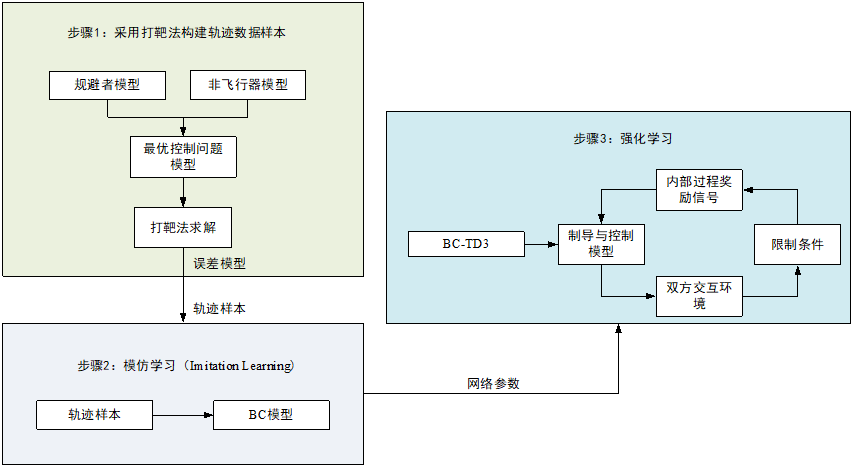
\includegraphics[width=0.82\linewidth]{fig02}
\caption{BC-TD3网络架构图}
\label{fig:bctd3-arch}
\end{figure}
BC-TD3与TD3网络训练超参数如下表~\ref{tab:hyperparams}所示：

\begin{table}[htbp]
\centering
\caption{TD3与BC-TD3训练超参数}
\label{tab:hyperparams}
\small
\begin{tabularx}{\linewidth}{lXX}
\toprule
超参数 & TD3 & BC-TD3 \\
\midrule
总训练步数 & 300 000 & 300 000 \\
学习率 & 1$\times$$10^{-4}$ & 1$\times$$10^{-4}$ \\
批次大小 & 256 & 256 \\
折扣因子 $\gamma$ & 0.99 & 0.99 \\
软更新系数 $\tau$ & 0.005 & 0.005 \\
经验回放容量 & 300 000 & 300 000 \\
开始更新步数 & 1 000 & 0 \\
训练频率 & 1 步 & 1 步 \\
策略延迟更新 & 3 & 3 \\
网络结构 & [256, 256] & [256, 256] \\
探索噪声 $\sigma$ & 0.1 & 0.1 \\
目标策略噪声 & 0.2 & 0.2 \\
目标噪声裁剪 & 0.5 & 0.5 \\
梯度裁剪 & ±10 & ±10 \\
BC 预填充比例 & — & 0.33 \\
BC 正则初始系数 $\lambda$$_0$ & — & 1.0 \\
BC 衰减步数 & — & 200 000 \\
\bottomrule
\end{tabularx}
\end{table}
\FloatBarrier
\subsubsection{BC-TD3算法网络训练}
完整离线训练流程如下：

\begin{algorithm}[H]
\caption{面向制导参数优化的 BC-TD3 离线训练}
\label{alg:bctd3}
{\footnotesize
\raggedright
输入：专家数据集 \(\mathcal{D}_{\text{expert}}\)，交会仿真器 \(\text{Env}\)\\
输出：训练后的 Actor \(\pi_\phi\)\\
// 阶段 1：BC 预训练\\
1: 以随机权重初始化 Actor \(\pi_\phi\)\\
2: for epoch = 1 to \(E_{\text{BC}}\) do\\
3:   从 \(\mathcal{D}_{\text{expert}}\) 采样小批量 \(\{(\boldsymbol{s}_n, \boldsymbol{a}_n)\}\)\\
4:   通过最小化 \(\mathcal{L}_{\text{BC}}\) 更新 \(\phi\)（式 \ref{eq:78}）\\
5: end for\\
6: 用 \(\mathcal{D}_{\text{expert}}\) 预填回放缓冲区 \(\mathcal{R}\)\\
// 阶段 2：TD3 微调\\
7: 初始化 Critic \(\psi_1, \psi_2\)，目标网络 \(\phi' \leftarrow \phi\)，\(\psi_j' \leftarrow \psi_j\)\\
8: for episode = 1 to \(E_{\text{TD3}}\) do\\
9:   将 Env 重置为随机初始条件 \(\boldsymbol{s}_0\)\\
10:  for \(n = 0, 1, 2, \ldots\) do\\
11:    \(\boldsymbol{a}_n = \pi_\phi(\boldsymbol{s}_n) + \boldsymbol{\eta}_n\)                    // 式 \ref{eq:84}\\
12:    在 Env 中执行 \(\boldsymbol{a}_n\) \(\to\) 由式 \eqref{eq:66} 得到 \(\boldsymbol{u}_A^*(t)\)\\
13:    观测 \(\boldsymbol{s}_{n+1}, r_n\)（式 \ref{eq:74}--\ref{eq:75}）\\
14:    将 \((\boldsymbol{s}_n, \boldsymbol{a}_n, r_n, \boldsymbol{s}_{n+1})\) 存入 \(\mathcal{R}\)\\
15:    从 \(\mathcal{R}\) 采样 \(N\) 条转移的小批量\\
16:    计算目标 \(y_n\)（式 \ref{eq:79}--\ref{eq:80}）\\
17:    通过最小化 \(\mathcal{L}_{\text{Critic}}\) 更新 Critic \(\psi_1, \psi_2\)（式 \ref{eq:81}）\\
18:    if \(n \mod d = 0\) then                                           // 延迟更新\\
19:      通过策略梯度更新 Actor \(\phi\)（式 \ref{eq:82}）\\
20:      软更新目标网络：\(\phi', \psi_j'\)（式 \ref{eq:83}）\\
21:    end if\\
22:  end for\\
23: end for\\
// 部署（在线推理）\\
24: return \(\pi_\phi\) — 每个制导周期：\(\boldsymbol{a} = \pi_\phi(\boldsymbol{s})\)，将 \(\boldsymbol{a}\) 与辨识矩阵送入式 \eqref{eq:66}
}
\end{algorithm}

\section{仿真结果}
\subsection{仿真条件}
本节评估了在三维规避者与双非合作飞行器交会下，提出的一体化最优规避-制导律与BC-TD3参数优化。本研究分为三个部分。第6.1节总结了仿真条件，包括交会几何、飞行器模型、训练设置与成功判据。第6.2节考察了无噪声环境下的规避和制导表现，重点关注学习效率、代表性轨迹以及蒙特卡洛成功率，比较经典和基于学习的基线。第6.3节进一步评估闭环在测量噪声下的鲁棒性，并比较BC-TD3带在线参数识别和不带在线参数识别的方案，以量化第3节开发的稀疏FF-RLS模块的优势。

所有仿真均在三维四体交会中进行：规避方到达固定目标同时躲避两枚非合作飞行器。非合作飞行器采用了具有相同性能参数的经典比例导引（PN）（假设1、2）。规避者加速度命令由闭环制导定律\eqref{eq:66}生成，其制导权重${\mathbf{p}} = {[w,{\kern 1pt} \gamma ,{\kern 1pt} {w_T},{\kern 1pt} {w_E}]^T}$由训练后的BC-TD3模型在线给出。

除非另有说明，期望规避距离为${d^*} = 20{\kern 1pt} {\text{m}}$，非合作飞行器作用半径为6m，目标成功到达阈值为10m，制导周期为$\Delta t = 0.1{\kern 1pt} {\text{s}}$。

考虑两种互补评估设置。在无噪声设置（第6.2节）中，相对距离、视线角/角速度与姿态角假定精确，从而\eqref{eq:66}中的矩阵元素可由式\eqref{eq:13}与\eqref{eq:15}解析求得。在有噪声设置（第6.3节）中，机载视线角/角速度与航迹倾角/偏角按注记1a叠加高斯白噪声；稀疏FF-RLS辨识器再由相对运动学恢复所需参数。

首先进行代表轨迹性能测试与分析。随后的蒙特卡洛试验采用拉丁超立方采样（LHS）对多维初始条件空间抽样，并在所有对比方法使用相同随机种子的前提下，报告规避、目标到达与双重成功率。

代表轨迹规避者与非合作飞行器交会初始条件如下表~\ref{tab:init-traj}所示：

\begin{table}[htbp]
\centering
\caption{代表轨迹交会初始条件与场景参数}
\label{tab:init-traj}
\small
\begin{tabularx}{\linewidth}{lXXX}
\toprule
对象 & 初始位置/m & 初始航迹倾角 & 初始航迹偏角 \\
\midrule
规避者$A$ & (10000,6000,3500) & ${\theta _{A0}} =  - {20^ \circ }$ & ${\psi _{{V_A}0}} = {155^ \circ }$ \\
非合作飞行器${D_1}$ & (1000,0,0) & ${\theta _{D10}} = {40^ \circ }$ & ${\psi _{{V_{D1}}0}} =  - {20^ \circ }$ \\
非合作飞行器${D_2}$ & (-1000,0,0) & ${\theta _{D20}} = {40^ \circ }$ & ${\psi _{{V_{D2}}0}} =  - {20^ \circ }$ \\
\bottomrule
\end{tabularx}
\end{table}
为验证所提算法的有效性，我们将四种制导方法进行对比：（1）纯比例导引，取${K_A} = 4$；（2）正弦机动规避，加速度指令为${u_{Ay}} = {A_\omega }\cos (2\pi f(t - {t_0}))$, ${u_{Az}} = {A_\omega }\sin (2\pi f(t - {t_0}))$，其中$f$为频率，${t_0}$为规避启动时刻，取${A_\omega } = 54,f = 0.15$；（3）基于纯TD3的最优一体化规避导引律；（4）基于BC-TD3的最优一体化规避导引律（本文所提方法）。

蒙特卡洛参数分布及范围如下表~\ref{tab:mc-dist}所示：

\begin{table}[htbp]
\centering
\caption{蒙特卡洛参数分布及范围}
\label{tab:mc-dist}
\small
\begin{tabularx}{\linewidth}{lXX}
\toprule
参数 & 分布范围 & 分布方式 \\
\midrule
${q_{yi}}$ & $[{20^ \circ },{70^ \circ }]$ & 均匀分布 \\
${q_{zi}}$ & $[ - {20^ \circ },{20^ \circ }]$ & 均匀分布 \\
${\eta _{{y_{Ai}}0}},{\eta _{{y_{Di}}0}}$ & $[ - {15^ \circ },{15^ \circ }]$ & 正态分布$N(0,{6^2})$，均匀分布 \\
${\eta _{{z_{Ai}}0}},{\eta _{{z_{Di}}0}}$ & $[ - {10^ \circ },{10^ \circ }]$ & 正态分布$N(0,{6^2})$，均匀分布 \\
${r_{AD0}}$ & $[10.5,13.5]{\text{km}}$ & 均匀分布 \\
$\beta $ & $[ - 1.5,1.5]{\text{km}}$ & 均匀分布 \\
\bottomrule
\end{tabularx}
\end{table}
\subsection{不考虑测量噪声的规避与制导}
本小节在理想（无噪声）信息条件下验证所提出的 BC-TD3 制导规避–目标到达律。本小节由于制导矩阵可精确计算，方法间的性能差异主要归因于在线制导参数策略的质量，而非传感器/辨识误差。报告三项互补研究：(i) 纯TD3与BC-TD3学习方法的学习曲线；(ii) 以表~\ref{tab:init-traj}所示为初值的各规避方法三维交会轨迹及对各非合作飞行器的放大交会视图；(iii) 基于表~\ref{tab:mc-dist}的各方法蒙特卡洛成功率统计。

纯TD3与BC-TD3学习方法的学习曲线如下图~\ref{fig:reward}所示

\begin{figure}[htbp]
\centering
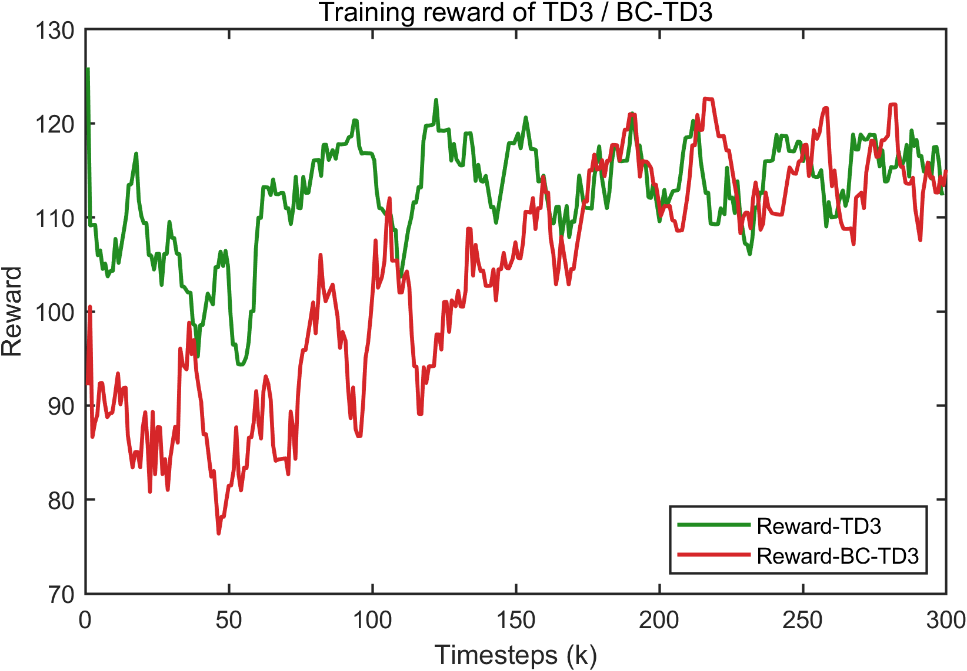
\includegraphics[width=0.92\linewidth]{fig03}
\caption{BC-TD3训练奖励曲线}
\label{fig:reward}
\end{figure}
各规避方法三维交会轨迹如下图~\ref{fig:traj-bctd3}--\ref{fig:traj-sine}所示：

\begin{figure}[htbp]
\centering
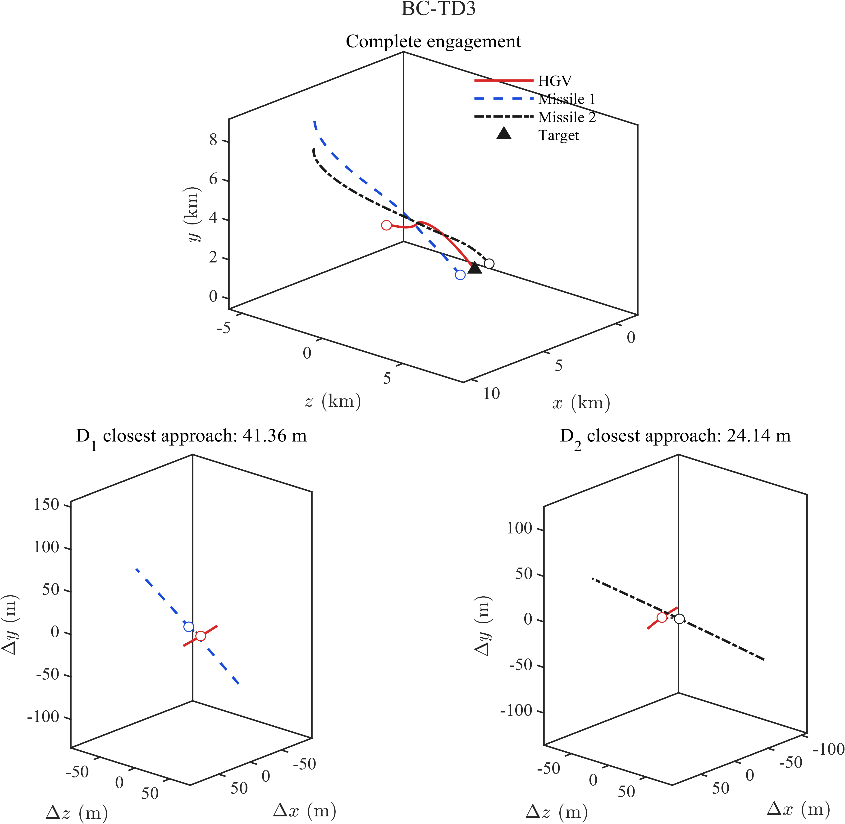
\includegraphics[width=0.92\linewidth]{fig04}
\caption{BC-TD3三维轨迹及与非合作飞行器交会局部放大图}
\label{fig:traj-bctd3}
\end{figure}
\begin{figure}[htbp]
\centering
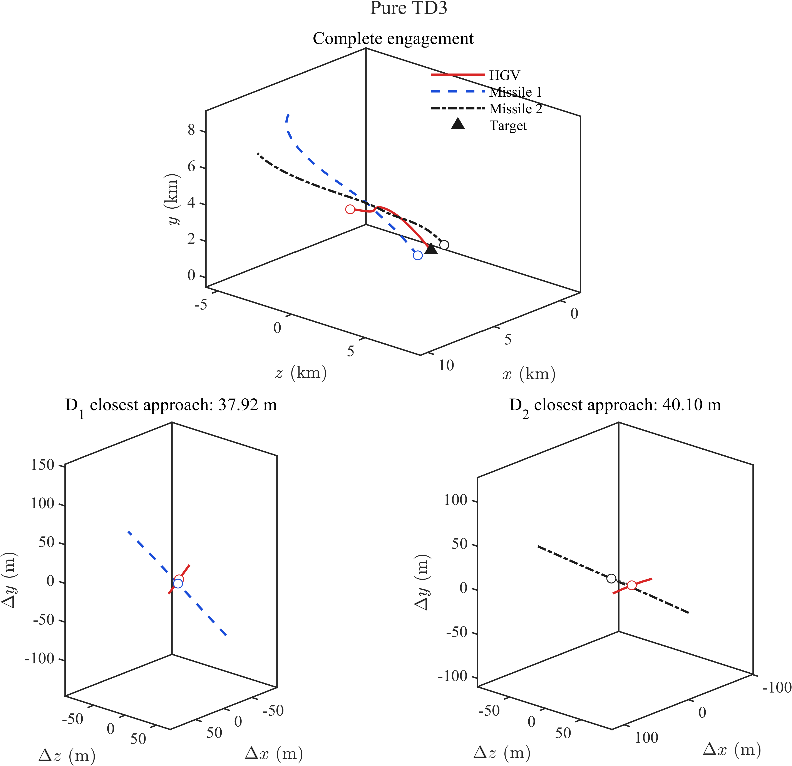
\includegraphics[width=0.92\linewidth]{fig05}
\caption{TD3三维轨迹及与非合作飞行器交会局部放大图}
\label{fig:traj-td3}
\end{figure}
\begin{figure}[htbp]
\centering
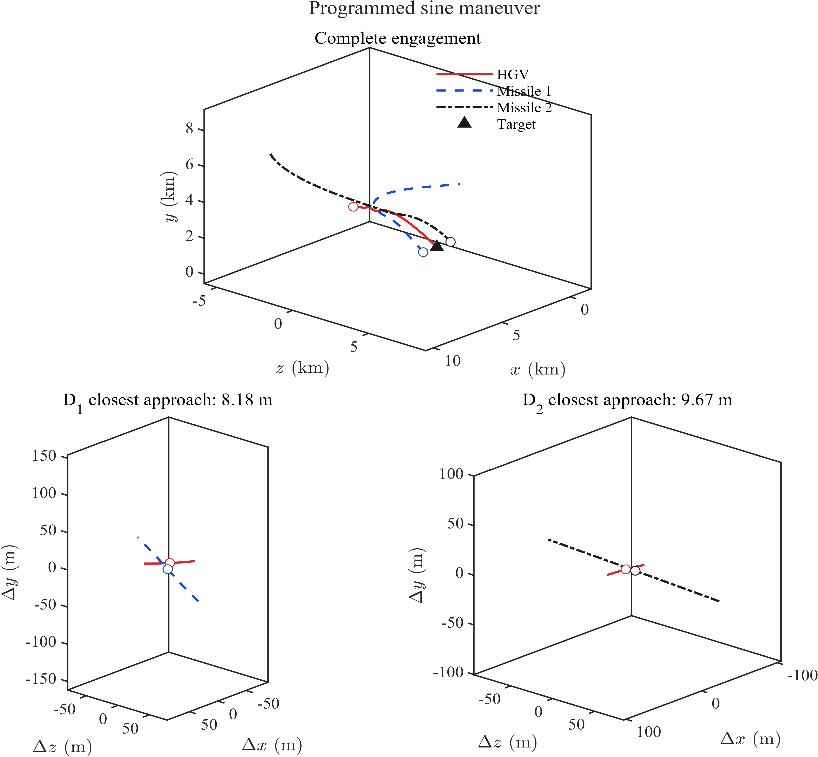
\includegraphics[width=0.92\linewidth]{fig06}
\caption{正弦机动方法三维轨迹及与非合作飞行器交会局部放大图}
\label{fig:traj-sine}
\end{figure}
四种制导方法加速度曲线如下图~\ref{fig:acc}所示：

\begin{figure}[htbp]
\centering
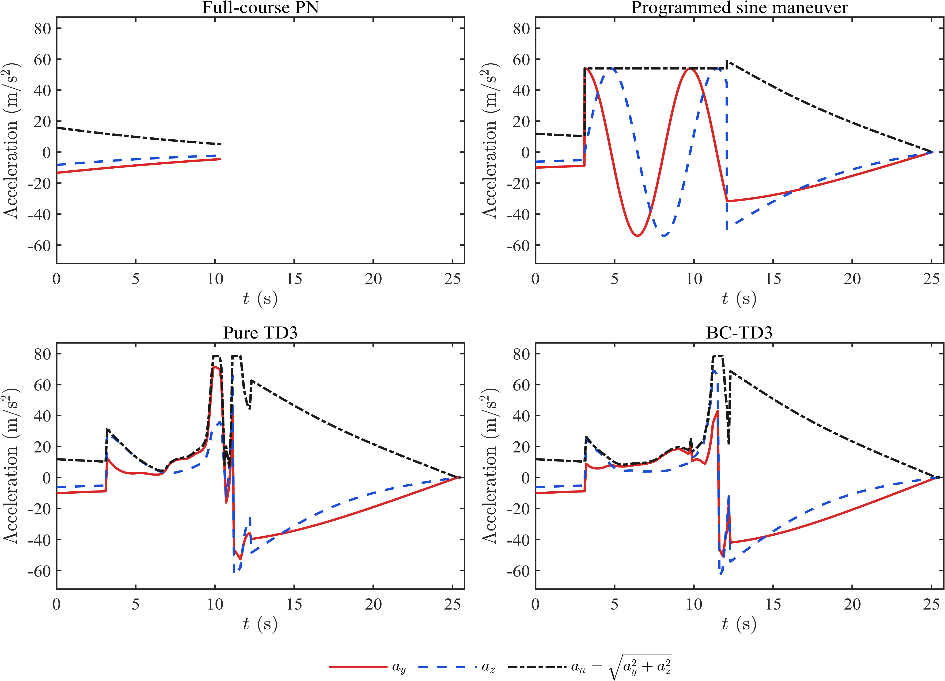
\includegraphics[width=0.92\linewidth]{fig07}
\caption{各方法法向加速度曲线}
\label{fig:acc}
\end{figure}
四种制导方法${r_{AD1}},{r_{AD2}},{r_{AT}}$变化如下图~\ref{fig:range}所示：

\begin{figure}[htbp]
\centering
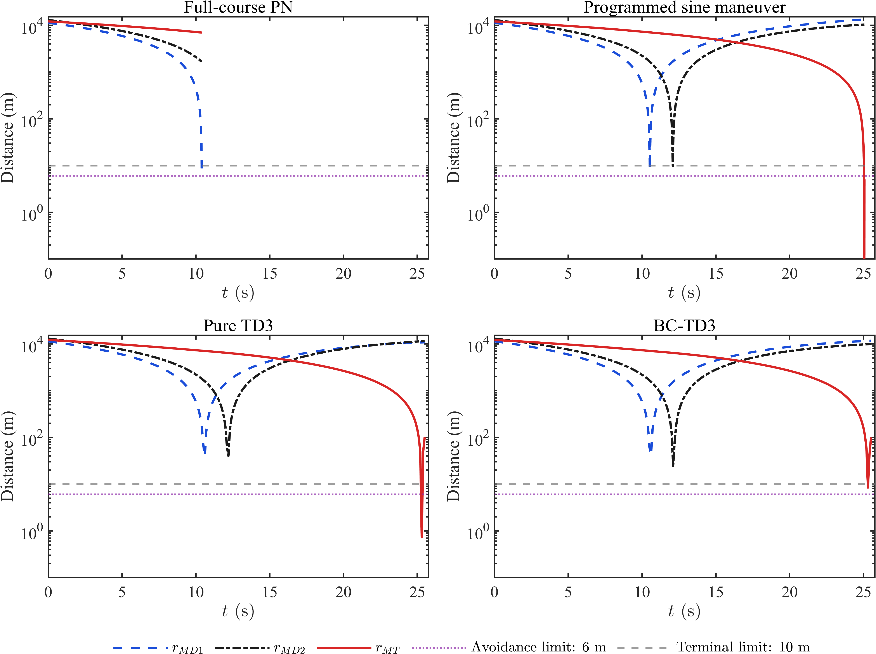
\includegraphics[width=0.92\linewidth]{fig08}
\caption{规避者与两非合作飞行器、目标间距离变化曲线}
\label{fig:range}
\end{figure}
由图~\ref{fig:acc}--\ref{fig:range}，全程比例制导时，规避方近似平飞、过载较小，约在10.5s时${r_{AD1}}$触及规避门限（6m），规避失败，仿真提前终止，未能完成目标到达制导。正弦程序机动在中段实施持续大幅正弦过载，${a_n}$长期维持在较高水平；${r_{AD1}}$, ${r_{AD2}}$最小距离均略高于6 m，末段${r_{AT}}$降至10 m以下，可同时完成规避与目标到达，但与非合作飞行器的安全余量较小。纯TD3与BC-TD3在中段自适应增大机动，约在10–12 s附近${a_n}$达到饱和（约80 m/s$^{2}$），随后过载逐渐回落至末端制导；二者的${r_{AD1}}$, ${r_{AD2}}$最小距离明显高于程序机动，且末端${r_{AT}}$均低于10 m，表明均可完成双飞行器规避与目标到达制导，其中BC-TD3的机动过程更为平滑、稳定。

为了比较性能，对BC+TD3、TD3、纯比例导引和程序机动规避策略进行了300次蒙特卡洛仿真，比较表列于表~\ref{tab:perf-nonoise}。

\begin{table}[htbp]
\centering
\caption{算法表现比较（不考虑噪声）}
\label{tab:perf-nonoise}
\small
\begin{tabularx}{\linewidth}{lXX}
\toprule
方法 & 双飞行器规避成功率$\min ({r_{AD1}},{r_{AD2}}) \geqslant 6{\text{m}}$ & 目标到达成功率（规避成功+${r_{AT,end}} \leqslant 10{\text{m}}$） \\
\midrule
仅对目标比例导引 & 0.0\% & 0.0\% \\
程序机动（正弦机动） & 76.3\% & 74.3\% \\
纯TD3 & 93.7\% & 93.0\% \\
BC+TD3 & 94.7\% & 94.3\% \\
\bottomrule
\end{tabularx}
\end{table}
规避方在不实施机动或仅采用固定程序机动时，难以同时完成双飞行器规避与目标到达。仅对目标比例制导时，双飞行器规避成功率与目标到达成功率均为0.0\%；正弦程序机动虽可将两项指标分别提升至76.3\%与74.3\%，但仍明显不足。纯TD3与BC+TD3均能较好完成规避与目标到达制导任务：纯TD3的规避成功率和目标到达成功率分别为93.7\%与93.0\%，而BC+TD3进一步达到 94.7\% 与 94.3\%。相比之下，BC+TD3 在两项成功率上均优于纯 TD3，综合表现更优，工程适用性也更好。

\subsection{考虑测量噪声的规避与制导}
在实际交会中，制导律\eqref{eq:66}所需的矩阵元素无法由无噪声运动学求得。按注记1a，机载视线角、视线角速度与姿态角叠加高斯白噪声；将这些测量代入式\eqref{eq:13}与\eqref{eq:15}会引入有偏且相互相关的矩阵误差。因此本小节在传感器噪声下重复上述交会研究，并考察第3节稀疏FF-RLS辨识器能否恢复闭环性能。给出两类结果：(i) 考虑噪声时在线辨识的典型BC-TD3轨迹及放大交会视图；(ii) 五种策略的蒙特卡洛对比，包括无辨识与有辨识的BC-TD3、TD3、正弦机动和纯PN。

图~\ref{fig:traj-id}给出了BC-TD3结合在线稀疏FF-RLS辨识时的典型有噪声飞行轨迹，初值基于表~\ref{tab:init-traj}，取噪声强度为${\sigma _q} = {0.3^ \circ }$，${\sigma _{\dot q}} = 0.003{\text{rad/s}}$，${\sigma _\theta } = {0.3^ \circ }$，${\sigma _\psi } = {0.3^ \circ }$。

\begin{figure}[htbp]
\centering
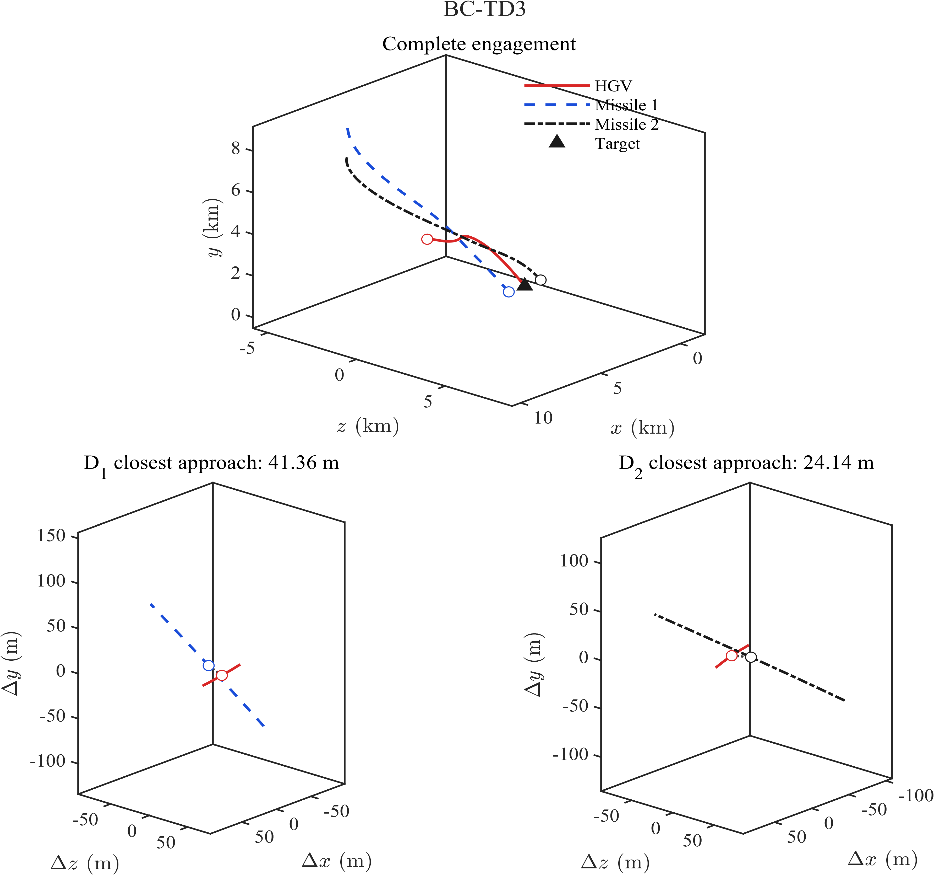
\includegraphics[width=0.92\linewidth]{fig09}
\caption{带辨识BC-TD3三维轨迹及交会局部放大图（含测量噪声）}
\label{fig:traj-id}
\end{figure}
未结合在线稀疏FF-RLS辨识时的典型有噪声飞行轨迹如下图~\ref{fig:traj-noid}所示：

\begin{figure}[htbp]
\centering
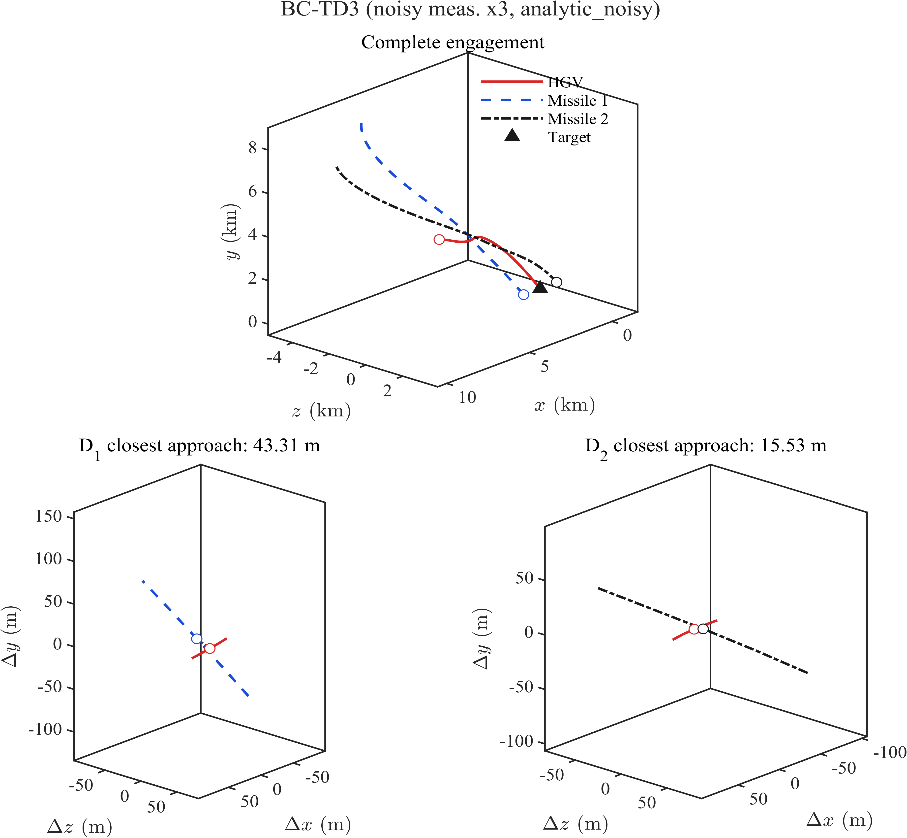
\includegraphics[width=0.92\linewidth]{fig10}
\caption{未带辨识BC-TD3三维轨迹及交会局部放大图（含测量噪声）}
\label{fig:traj-noid}
\end{figure}
由图~\ref{fig:traj-id}--\ref{fig:traj-noid}，加入上述测量噪声并经在线稀疏FF-RLS辨识后，整体制导与飞行过程几乎未受影响：规避方仍能完成大范围机动并准确抵达目标，均保持有效规避。相比之下，未引入辨识时，测量噪声会直接进入制导回路，最近规避距离分别为43.31 m和15.53 m，可以明显看出对第二个非合作飞行器${D_2}$的规避距离明显下降，末端目标到达精度也受到一定程度的影响。可见，在没有在线稀疏 FF-RLS辨识的情况下存在规避和目标到达性能下降的情况，加入辨识可有效抑制测量噪声对规避与目标到达制导的干扰。

考虑测量噪声的蒙特卡洛测试结果如下表~\ref{tab:perf-noise}所示：

\begin{table}[htbp]
\centering
\caption{算法表现比较（考虑噪声）}
\label{tab:perf-noise}
\small
\begin{tabularx}{\linewidth}{lXX}
\toprule
方法（未特殊标注则不带辨识） & 双飞行器规避成功率$\min ({r_{AD1}},{r_{AD2}}) \geqslant 6{\text{m}}$ & 目标到达成功率（规避成功+${r_{AT,end}} \leqslant 10{\text{m}}$） \\
\midrule
仅对目标比例导引 & 0.0\% & 0.0\% \\
程序机动（正弦机动） & 76.3\% & 74.3\% \\
纯TD3 & 92.3\% & 91.7\% \\
BC+TD3 & 93.7\% & 93.3\% \\
带辨识BC+TD3 & 96.7\% & 96.0\% \\
\bottomrule
\end{tabularx}
\end{table}
在考虑测量噪声的条件下，规避方在不实施机动或仅采用固定程序机动时，仍难以同时完成双飞行器规避与目标到达。仅对目标比例制导时，双飞行器规避成功率与目标到达成功率均为0.0\%；正弦程序机动虽可将两项指标分别提升至76.3\% 与 74.3\%，但仍明显不足。纯TD3与BC+TD3的规避成功率和目标到达成功率分别为92.3\%、91.7\%与93.7\%、93.3\%，虽可较好完成任务，但受噪声影响较无噪声情形略有下降。引入在线稀疏FF-RLS 参数辨识后，带辨识 BC+TD3将两项成功率进一步提升至96.7\%与96.0\%，显著优于未辨识的BC+TD3，表明参数辨识可有效抑制测量噪声干扰，提升规避与目标到达制导的稳健性。


\section{结论}
本文针对规避者需同时规避两枚非合作飞行器并保持对指定目标终端精度的需求，提出了一种三维一体化规避制导框架。建立了四体相对运动模型，用以描述规避者、目标与两枚非合作飞行器之间的耦合交互。在此基础上，将双非合作飞行器规避需求、目标到达精度与控制能耗惩罚纳入统一性能指标，推导了最优闭环制导律。该制导律显式计入交叉耦合效应，即一次机动同时影响两次规避交会与终端目标到达。

为在不同交会几何下自适应选择制导权重，提出了基于BC-TD3的参数优化策略。利用单打靶优化方法生成的专家示范对策略进行初始化，再经TD3微调提升其在非线性多约束环境中的适应能力。此外，引入带稀疏正则化与遗忘因子的递推最小二乘辨识器，从含噪测量中估计状态空间模型的非平凡参数，从而降低制导回路对测量误差的敏感性。

仿真结果表明，所提方法能够在三维双非合作飞行器场景中可靠地同时完成规避与目标到达。在无噪声蒙特卡洛试验中，BC-TD3的规避成功率与目标到达成功率分别为94.7\%和94.3\%，优于传统比例导引、程序正弦机动以及不含行为克隆的TD3。在测量噪声条件下，引入稀疏在线辨识后，两项成功率进一步提高至96.7\%和96.0\%。上述结果表明，所提框架可为多非合作飞行器一体化规避与终端制导提供有效且鲁棒的解决方案。后续工作将进一步考虑更贴近实际的飞行器动力学、异构及机动非合作飞行器、执行机构约束，以及更广泛不确定性条件下的验证。


\printbibliography[title={参考文献}]
\end{document}
